\newcommand{\lang}{ngerman}

\ifdefined\ishandout
\newcommand{\handoutmode}{handout}
\else
\newcommand{\handoutmode}{}
\fi


\documentclass[10pt,
\lang ,
\handoutmode ,
compress
]{beamer}
% Für den Header
% Modify for different languages
\usepackage{ifthen}

\newcommand{\unibastring}{\ifthenelse{\equal{\lang}{ngerman}}{Universit\"at Bamberg}{University of Bamberg}}

%\usepackage{doc} %for \BibTex but causes lots of errors...
\usepackage{eurosym}
\usepackage{etex}
\usepackage{ulem}
\usepackage{stmaryrd}
\usetheme{UniBa}
%\usefonttheme{
%	default | professionalfonts | serif |
%	structurebold | structureitalicserif |
%	structuresmallcapsserif
%}
\usefonttheme{professionalfonts}
%\useinnertheme{
%	circles | default | inmargin |
%	rectangles | rounded
%}
\useinnertheme{rectangles}
%\useoutertheme{
%	default | infolines | miniframes |
%	shadow | sidebar | smoothbars |
%	smoothtree | split | tree
%}
%\useoutertheme{split}
\setbeamercovered{transparent}

% Without navigation symbols
\beamertemplatenavigationsymbolsempty

%% Formatierungen
\usepackage{url}
\usepackage{latexsym}			% schönere Symbole
\usepackage{color}
%\usepackage{float}

%% Zeichensätze
\usepackage[utf8]{inputenc}
\usepackage{lmodern}
\usepackage{float}
%\usepackage{thumbpdf}
\usepackage{wasysym}
%\usepackage{ucs}

%Meta info
%Necessary Information
\author[V. Barth, M. Gromowski, J. Karp, J. Rabold, L. Schatt, M. Tr\"ager]{{\small Valentin Barth, Mark Gromowski, Jascha Karp, Johannes Rabold, \newline Lisa Schatt, Michael Träger}}
\title{\LaTeX ~-Tutorial by Fachschaft WIAI}
%The day of the presentation
\date{April 6, 2016}

%Optional Information
\subject{subject}
\keywords{keywords}

%Already set
\ifthenelse{\equal{\lang}{ngerman}}{%
\institute[FS WIAI]{Fachschaft WIAI (Informational Systems and Applied Computer Sciences)\\ of Otto Friedrich University Bamberg}}{%
\institute[KTR]{Professorship for Computer Science,\\%
        Communication Services, Telecommunication Systems and Computer Networks}}

\titlegraphic{
\includegraphics[width=13mm,height=13mm]{image/logo}}


%% Hyperref
\usepackage{hyperref}

\makeatletter
\hypersetup{pdftitle={\@title}, pdfauthor={\@author}, linktoc=page, pdfborder={0 0 0 [3 3]}, breaklinks=true, linkbordercolor=unibablueI, menubordercolor=unibablueI, urlbordercolor=unibablueI, citebordercolor=unibablueI, filebordercolor=unibablueI}
\makeatother
%% Define a new 'leo' style for the package that will use a smaller font.
\makeatletter
\def\url@leostyle{%
  \@ifundefined{selectfont}{\def\UrlFont{\sf}}{\def\UrlFont{\small\ttfamily}}}
\makeatother
%% Now actually use the newly defined style.
\urlstyle{leo}

%% Sprache
\ifthenelse{\equal{\lang}{ngerman}}{\usepackage[ngerman]{babel}}{\usepackage[\lang]{babel}}

% Abbildung -> Abb.
\addto\captionsngerman{\renewcommand{\figurename}{Abb.}}

%}
%%\usepackage{abstract}

%% Mathe und Formeln
\usepackage{calc}
\usepackage{amsmath}
\usepackage{amssymb,amsthm,amsfonts}
\usepackage{dsfont}
\usepackage[nice]{nicefrac}
\usepackage{cancel}  %%druchstreichen von Formeln
%
%% Programmieren mit Latex
\usepackage{ifthen}


\usepackage{dirtree}   %setzen von baumstrukturen

%%%   Fuer anspruchsvolle Tabellen   %%
\usepackage{longtable, colortbl}
\usepackage{multicol, multirow}
%
%%%  Für Grafiken %%
\usepackage{graphicx}
\usepackage{tikz}
%\usepackage{pgfplots}
\usetikzlibrary{calc,arrows,fit,positioning,trees,backgrounds,shadows,decorations,decorations.markings,decorations.shapes,shapes,patterns,fadings}
\usepackage[font=footnotesize]{subfig}


\makeatletter
\newcount\dirtree@lvl
\newcount\dirtree@plvl
\newcount\dirtree@clvl
\def\dirtree@growth{%
  \ifnum\tikznumberofcurrentchild=1\relax
  \global\advance\dirtree@plvl by 1
  \expandafter\xdef\csname dirtree@p@\the\dirtree@plvl\endcsname{\the\dirtree@lvl}
  \fi
  \global\advance\dirtree@lvl by 1\relax
  \dirtree@clvl=\dirtree@lvl
  \advance\dirtree@clvl by -\csname dirtree@p@\the\dirtree@plvl\endcsname
  \pgf@xa=1cm\relax
  \pgf@ya=-1cm\relax
  \pgf@ya=\dirtree@clvl\pgf@ya
  \pgftransformshift{\pgfqpoint{\the\pgf@xa}{\the\pgf@ya}}%
  \ifnum\tikznumberofcurrentchild=\tikznumberofchildren
  \global\advance\dirtree@plvl by -1
  \fi
}

\tikzset{
  dirtree/.style={
    growth function=\dirtree@growth,
    every node/.style={anchor=north},
    every child node/.style={anchor=west},
    edge from parent path={(\tikzparentnode\tikzparentanchor) |- (\tikzchildnode\tikzchildanchor)}
  }
}
\makeatother
%\usepackage{fp}
%
%%%  Zur Darstellung des Euro-Symbols   %%
%\usepackage{eurosym, wasysym}
%\selectlanguage{german}
%
%%%   Fuer Bibtex nach APA Style (American Psychology Association)   %%
%\usepackage[numbers]{natbib}
\usebibitemtemplate{\insertbiblabel}

%% Code-Hervorhebung
%% Quellcode

%\usepackage[numbered,autolinebreaks,useliterate]{mcode}
\usepackage{verbatim}            % Quellcode einbinden (\verbatiminput) standardpaket
%\usepackage{moreverb} 
%% PseudoCode
%\usepackage{algorithm}
\usepackage{algpseudocode}
%%\usepackage{algorithmicx}
%%\floatname{algorithm}{Algorithmus}
%\algrenewcommand{\algorithmiccomment}[1]{\hskip1em\textcolor{gray!60}{$\rhd$ #1}}
%%\renewcommand{\listalgorithmname}{Algorithmen}
%%\def\algorithmautorefname{Algorithmus}
%
%%% Code Highlighting
%\definecolor{mygray}{gray}{.75}
\usepackage{listings} 
%\lstset{numbers=left, numberstyle=\tiny, numbersep=6pt} 
%\lstset{language=Python}
%\lstset{classoffset=1, morekeywords={mycontext}, keywordstyle=\color{darkgreen}, classoffset=0, keywordstyle=\color{darkblue}}
%\lstset{basicstyle=\small, showstringspaces=false, commentstyle=\color{mygray}, breaklines=true, captionpos=b}
%\renewcommand{\lstlistingname}{Code-Ausschnitt}
%\renewcommand{\lstlistlistingname}{Code-Ausschnitte}
%\def\lstlistingautorefname{Code-Ausschnitt}


%%%%%%%%%%%%%%%%%%%%%%%%%%%%%%%%%%%%%%%%%%%%%%%%%%%%%%%%%%%%%%%%%%%%%%%%%%%%%%%%%%%%%%%%%%%%
%%%                                   COMMAND SETUP                                       %%
%%%%%%%%%%%%%%%%%%%%%%%%%%%%%%%%%%%%%%%%%%%%%%%%%%%%%%%%%%%%%%%%%%%%%%%%%%%%%%%%%%%%%%%%%%%%

%#1 Breite
%#2 Datei (liegt im image Verzeichnis)
%#3 Beschriftung
%#4 Label fuer Referenzierung
\newcommand{\image}[4]{
\begin{figure}[H]
\centering
\includegraphics[width=#1]{#2}
\caption{\footnotesize{#3}}
\label{#4}
\end{figure}
}

% #1 videofile
% #2 scalefactor
\newcommand{\video}[2]{%
\includemovie[text={\includegraphics[scale=#2]{praesi/video/#1.png}}, autoplay, mouse=true, repeat=1]{}{}{praesi/video/#1.swf}}


\def\signed #1{{\leavevmode\unskip\nobreak\hfil\penalty50\hskip2em
  \hbox{}\nobreak\hfil(#1)%
  \parfillskip=0pt \finalhyphendemerits=0 \endgraf}}

\newsavebox\mybox
\newenvironment{aquote}[1]
  {\savebox\mybox{#1}\begin{fancyquotes}}
  {\signed{\usebox\mybox}\end{fancyquotes}}


\hyphenation{op-tical net-works semi-conduc-tor}

\setbeamertemplate{caption}[numbered]
%\numberwithin{figure}{section}
\begin{document}

\frame{\titlepage}

\AtBeginSection[]
{
  \frame<handout:0>
  {
    \frametitle{Outline}
    \begin{multicols}{2}
    \tableofcontents[currentsection,hideallsubsections]
    \end{multicols}
  }
}

%\AtBeginSubsection[]
%{
%  \frame<handout:0>
%  {
%    \frametitle{Outline}
%    \tableofcontents[sectionstyle=show/hide,subsectionstyle=show/shaded/hide,subsubsectionstyle=hide]
%  }
%}

%\AtBeginSubsubsection[]
%{
%  \frame<handout:0>
%  {
%    \frametitle{Outline}
%    \tableofcontents[sectionstyle=show/hide,subsectionstyle=show/shaded/hide,subsubsectionstyle=show/shaded/hide]
%  }
%}

\newcommand<>{\highlighton}[1]{%
  \alt#2{\structure{#1}}{{#1}}
}

\newcommand{\icon}[1]{\pgfimage[height=1em]{#1}}

\begin{frame}
\frametitle{\"Uber dieses Tutorium}
%\begin{block}{"Uber dieses Tutorium}
\begin{itemize}
\item Powered by Prof.\,Dr.\,Udo Krieger
\item In Version 10 überarbeitet und erweitert von Michael Träger und Valentin Barth (mit Unterstützung von Michael Timpelan)
\item Version 9 in \LaTeX -Beamer gesetzt und erweitert von Linus Dietz
\item Ursprünglicher Foliensatz von\begin{itemize}
\item Marcel Grossmann
\item Steffen Illig
\item Martin Sticht
\item Michael Timpelan
\end{itemize}
\item ca. 2600 Zeilen Code
\item Quelltext auf GitHub: \url{https://github.com/fs-wiai/LaTeX-Tutorial}
\end{itemize}
%\end{block}
\end{frame}

\frame<handout:0>
 {
%  \addtocounter{framenumber}{-1}
 	\frametitle{Zeitplan}
    \begin{itemize}
	    \item Mittagspause: ca. 12 Uhr (etwa 45 Minuten)
	    \item Ende: ca. 15:30 Uhr
	    \medskip
	    %TODO auch erwähnen?
	    \item[] Anschließend: Spezielle Fragen und individuelle Beratung %zu bereits von euch verfassten Dokumenten
    \end{itemize}
 }

 \frame<handout:0>
  {
 %  \addtocounter{framenumber}{-1}
  	\frametitle{Vorstellung}
     \begin{itemize}
 	    \item Wer sind wir?
 	    \begin{itemize}
        \item \textbf{Anika Amma} (Bachelor Angewandte Informatik)
        \item \textbf{Andreas Erhard} (Master Angewandte Informatik)
        \item \textbf{Florian Knoch} (Bachelor Software Systems Science)
        \item \textbf{Fabian Lamprecht} (Bachelor Angewandte Informatik)
        \item \textbf{Martin Müller} (Master Angewandte Informatik)
        \item \textbf{Johannes Rabold} (Master Angewandte Informatik)
        \item \textbf{Michael Träger} (Master Angewandte Informatik)
 	    \end{itemize}
 	    \medskip
 	    \item Wer seid ihr?
 	    \begin{itemize}
	 	    \item Fakultät
	 	    \item Studiengang
	 	    \item Semester
 	    \end{itemize}
     \end{itemize}
  }

\begin{frame}{\contentsname}
    \frametitle{Outline}
\begin{multicols}{2}
\tableofcontents[hideallsubsections]
\end{multicols}
\end{frame}


%%%%%%%%%%%%%%%%%%%%%%%%%%%%%%%%%%%%%%%%%
%%%%%%%%%% Content starts here %%%%%%%%%%
%%%%%%%%%%%%%%%%%%%%%%%%%%%%%%%%%%%%%%%%%
%\input{content/spielwiese}
\section{Intro} 

\subsection{Anwendungsbereiche, Sinn \& Zweck}
\begin{frame}[t]
\frametitle{Einf\"uhrung}
\framesubtitle{Sinn -- Unsinn -- Wahnsinn}
\bigskip
\bigskip
\bigskip

\begin{columns}[t]
\begin{column}{.3\textwidth}
\textbf{Sinnvoll}\\[3mm]
\begin{itemize}
\item wissenschaftliche Arbeiten
\item Bücher
\item Lebenslauf \& Bewerbungen
\end{itemize}
\end{column}
\begin{column}{.30\textwidth}
\textbf{Unsinn}\\[3mm]
\begin{itemize}
\item private Briefe
\item Geburtstags-einladungen
\item Getr"ankekarten
\end{itemize}
\end{column}
\begin{column}{.3\textwidth}
\textbf{Wahnsinn}\\[3mm]
\begin{itemize}
\item Einkaufszettel
\item Brainstorming
\item \ldots 
\end{itemize}
\end{column}
\end{columns}
\end{frame}

%-------------------------------------------------------------------------------

\begin{frame} 
\frametitle{Vom Code zum Dokument}
\framesubtitle{Kein WYSIWYG} 
\begin{columns}
\begin{column}{.7\textwidth}
\image{\textwidth}{image/worddoc.jpg}{\textbf{W}hat \textbf{Y}ou \textbf{S}ee \textbf{I}s \textbf{W}hat \textbf{Y}ou
\textbf{G}et}{img:worddoc}
\end{column}
\begin{column}{.3\textwidth}
\image{\textwidth}{image/codescreen.png}{What Will I Get?}{img:codescreen}
%% Compile Animation
\end{column}
\end{columns}
\end{frame}

%-------------------------------------------------------------------------------

\begin{frame}
\frametitle{Einf\"uhrung}
\framesubtitle{Vorgehensweise}
\begin{columns}[onlytextwidth]
\begin{column}{0.40\textwidth}
\image{.8\textwidth}{image/codescreen.png}{Textdatei mit \LaTeX ~-Code}{img:code}
\end{column}
\begin{column}{0.25\textwidth}
\image{.8\textwidth}{image/miktex.jpg}{Compiler (z.B. MikTeX)}{img:miktex}
\end{column}
\begin{column}{0.25\textwidth}
\image{.6\textwidth}{image/pdflogo.png}{Sch\"ones, lesbares und druckbares Dokument}{img:pdf}
\end{column}
\end{columns}
\end{frame}


%-------------------------------------------------------------------------------

\subsection{Vorteile \& Nachteile}
\begin{frame}
\frametitle{Einf\"uhrung}
\framesubtitle{Vorteile \& Nachteile}
\textbf{Vorteile}
\begin{itemize}
\item  dynamische Verzeichnisse und Referenzen
\item  automatische Layouts
\item  einfaches verteiltes Arbeiten möglich
\end{itemize}

\textbf{Nachteile}
\begin{itemize}
\item  Was kommt später raus?
\item  viele, zum Teil komplexe Befehle
\end{itemize}
\end{frame}

%-------------------------------------------------------------------------------

\subsection{\LaTeX --Compiler}
\begin{frame}
\frametitle{Einf\"uhrung}
\framesubtitle{\LaTeX - Compiler}
\begin{columns}[t]
\begin{column}{.4\textwidth}
\textbf{Windows:}\\
\begin{itemize}
  \item MikTex (http://www.miktex.org)\\
   2 Varianten: Basic oder  Complete
  %\item ProTeXt (http://www.tug.org/protext)\\
enthält MikTex, TeXnicCenter und Ghostscript – einfache Installation\\
\end{itemize}
\end{column}
\begin{column}{.6\textwidth}
\textbf{Unix}
\begin{itemize}
  \item \textbf{Linux:} TeXLive\\
Pakete unter Ubuntu: {\ttfamily texlive-full} ist das Meta-Paket mit allen
ben\"otigten Paketen. Enthält auch folgende:
\begin{itemize}
  \item {\ttfamily texlive-base
  \item texlive-lang-german}
\end{itemize}
Installation: {\ttfamily sudo apt-get install texlive-full}
\item \textbf{MacOS:} MacTeX (http://www.tug.org/mactex/2009)\\
\end{itemize}
\end{column}
\end{columns}
\end{frame}

%-------------------------------------------------------------------------------

%\subsection{Freie Editoren}
%
%\subsubsection{*nix}
%\begin{frame}
%\frametitle{Einf\"uhrung}
%\framesubtitle{Freie Editoren -- Linus \& MacOS }
%\begin{itemize}
% \item Kile\footnote{http://kile.sourceforge.net/}\\KDE-Programm, auch unter Gnome\slash Unity etc.
% verwendbar. Installation auf Debiansystemen mit {\ttfamily sudo apt-get
% install kile}.
%  \item Vim \LaTeX -suite (Plugin)\footnote{http://vim-latex.sourceforge.net/}\\
%  Ein Traum f"ur Vim-User.
%  \item TexShop (MacOS)\footnote{http://pages.uoregon.edu/koch/texshop/}
%\end{itemize}
%\end{frame}

%-------------------------------------------------------------------------------

%\subsubsection{Windows}
%\begin{frame}
%\frametitle{Einf\"uhrung}
%\framesubtitle{Freie Editoren -- Windows}
%\begin{itemize}
%\item TeXnicCenter\footnote{http://www.texniccenter.org/}
%  %\item \ldots
%\end{itemize}
%\end{frame}

%-------------------------------------------------------------------------------

\subsubsection{Cross-Platform}
\begin{frame}
\frametitle{Einf\"uhrung}
\framesubtitle{Freie Editoren -- Cross-Platform}
\begin{itemize}
  \item TeXstudio\footnote{\url{http://sourceforge.net/projects/texstudio}}\\
  Sehr solide und mächtig, verwenden wir hier im Tutorium.
  \item TeXMaker\footnote{\url{http://www.xm1math.net/texmaker}}\\
   Grundlage von TeXstudio, etwas schlanker, wird kaum noch weiterentwickelt.
  \item TeXlipse\footnote{\url{http://texlipse.sourceforge.net}}\\ F"ur fortgeschrittene User, Plugin f"ur
  Eclipse. Gute IDE-Unterst\"utzung, Code-Completion, Autobuilds, Versionsverwaltung etc.
\end{itemize}
\end{frame}

%-------------------------------------------------------------------------------

\subsubsection{Online}
\begin{frame}
\frametitle{Online}
\framesubtitle{Multiediting -- auch Kollaborativ}
\begin{itemize}
  \item ShareLatex\footnote{\url{https://www.sharelatex.com}, \url{https://github.com/sharelatex}}\\
  Teilweise Open Source, Onlineversion kostenlos für Einzelbenutzer
  \item Overleaf\footnote{\url{https://www.overleaf.com}}\\
  Teilweise kostenpflichtig, hosted
  \item FlyLatex\footnote{\url{https://github.com/alabid/flylatex}}\\ 
  Open Source, weniger mächtig
  \item Viele Weitere ...
  \vspace{7mm}
  \item In der Uni wird auch oft git\footnote{\url{https://git-scm.com}} zur Synchronisation verwendet.
\end{itemize}
\end{frame}


%-------------------------------------------------------------------------------

\begin{frame}
%TODO texstudio!
\frametitle{TeXStudio}
\framesubtitle{\"Uberblick}
\image{\textwidth}{image/texstudio_overview.png}{Das Standardfenster von TeXStudio}{img:texstudio1}
\end{frame}

%-------------------------------------------------------------------------------

%\begin{frame}
%\frametitle{TeXmaker}
%\framesubtitle{Synctex}
%\image{\textwidth}{image/synctex.png}{Synctex}{img:synctex}

%\end{frame}

\begin{frame}
\frametitle{Mein erstes \LaTeX~-Dokument}
\begin{block}{Neue Befehle:}
\begin{itemize}
\item \begin{ttfamily}\color{nounibaredII}\textbackslash documentclass\color{nounibagreenI}\color{black}\{article\}\end{ttfamily}
\item \begin{ttfamily}\color{unibablueI}\textbackslash begin\color{black}\{document\}\end{ttfamily}
\item \begin{ttfamily} Inhalt als plain text \end{ttfamily}
\item \begin{ttfamily}\color{unibablueI}\textbackslash end\color{black}\{document\}\end{ttfamily}
\end{itemize}
\end{block}
Das ist alles was man f\"ur ein \LaTeX -Dokument braucht. Und das probieren wir jetzt aus!

\end{frame}

\documentclass{article}

\begin{document}
Hello World!
\end{document}


\section{Formatierung}

\begin{frame}
\frametitle{Ein erstes Anwendungsbeispiel}
\framesubtitle{\"Uberschriften, Inhaltsverzeichnis, einfache Formatierung,
Sonderzeichen}
\begin{block}{Neue Befehle in diesem Abschnitt}
\begin{multicols}{2}
\begin{itemize}
  \item \begin{ttfamily}\color{nounibaredI}\textbackslash usepackage\color{black}\{Paket\}
  \item \color{nounibaredI}\textbackslash befehl\color{nounibagreenI}[evtl\_optionen]\color{black}\{\\Formatierter Text\}
  \item \color{unibablueI}\textbackslash begin\color{black}\{Umgebung\}
  \item \color{unibablueI}\textbackslash end\color{black}\{Umgebung\}
  \item \color{nounibaredI}$\backslash\backslash$\color{black}
  \item \color{nounibaredI}\textbackslash newpage\color{black}
  \item \color{unibablueI}\textbackslash sub$^*$section\color{black}\{Titel\}
  \item $\color{nounibaredII}\backslash$\color{nounibaredI}textbf\color{black}\{Text\}
  \item $\color{nounibaredII}\backslash$\color{nounibaredI}textit\color{black}\{Text\}
  \item $\color{nounibaredII}\backslash$\color{nounibaredI}underline\color{black}\{Text\}
  \item \color{nounibaredI}$\color{nounibaredI}\backslash$tiny
  \item \color{nounibaredI}$\color{nounibaredI}\backslash$scriptsize
  \item \color{nounibaredI}$\color{nounibaredI}\backslash$footnotesize
  \item \color{nounibaredI}$\color{nounibaredI}\backslash$normalsize
  \item \color{nounibaredI}$\color{nounibaredI}\backslash$large
  \item \color{nounibaredI}$\color{nounibaredI}\backslash$Large
  \item \color{nounibaredI}$\color{nounibaredI}\backslash$LARGE
  \item \color{nounibaredI}$\color{nounibaredI}\backslash$huge\end{ttfamily}
\end{itemize}
\end{multicols}
\end{block}
\end{frame}

%-------------------------------------------------------

%TODO in erweiterung einbauen?
%\begin{frame}
%\frametitle{Ein erstes Anwendungsbeispiel}
%\framesubtitle{Pakete einbinden und Befehle anwenden}
%\begin{itemize}
%  \item Pakete sind Sammlungen von Befehlen oder enthalten z.B. Zeichensätze.\\ Sie werden zu
%  Beginn einer \TeX-Datei angegeben:\\
%  \smallskip
%\textbf{\begin{ttfamily}\color{nounibaredII}\textbackslash usepackage\color{black}\{babel\}
%
%\smallskip
%\end{ttfamily}}
% Einbinden des Paketes „\begin{ttfamily}babel\end{ttfamily}“. (F\"ur Internationalisierung)
%\item Schreibweise von Latex-Befehlen:
%
%\textbf{\begin{ttfamily}\color{nounibaredII}\textbackslash befehl\color{nounibagreenI}[evtl\_optionen]\color{black}\{Formatierter\_Text\}\end{ttfamily}}
%\begin{itemize}
%  \item in \begin{ttfamily}\{\}\end{ttfamily} stehen immer notwendige Parameter bzw. Text
% \item in \begin{ttfamily}[ ]\end{ttfamily} stehen (falls vorhanden)
% zus"atzliche, optionale Parameter
% \item zum Beispiel:
%
%
%\begin{ttfamily}
%\color{nounibaredII}\textbackslash documentclass\color{nounibagreenI}[a4paper,12pt,pdftex,ngerman]\color{black}\{article\}
%\end{ttfamily}
%\end{itemize}
%\end{frame}

%-------------------------------------------------------

\begin{frame}
\frametitle{Ein erstes Anwendungsbeispiel}
\framesubtitle{Befehle cont'd}
\begin{columns}
\begin{column}{0.55\textwidth}
\begin{ttfamily}\footnotesize
\color{nounibaredI}\color{nounibaredI}\textbackslash documentclass\color{black}\color{nounibagreenI}[a4paper, pdftex, ngerman]\color{black}\{article\} \\
\color{nounibaredI}\color{nounibaredI}\textbackslash usepackage\color{black}\color{nounibagreenI}[utf8]\color{black}\{inputenc\} \\
\color{nounibaredI}\color{nounibaredI}\textbackslash usepackage\color{black}\color{nounibagreenI}[T1]\color{black}\{fontenc\} \\
\color{nounibaredI}\color{unibablueI}\textbackslash\color{unibablueI}begin\color{black}\color{black}\{document\} \\
Das ist ein einfaches Minidokument \\
ohne Besonderheiten. Zeilenumbrüche \\
funktionieren immer automatisch! \\
Mehrere \\
Leerzeichen hintereinander werden  \\
zu einem zusammengefasst. \\
Getrennt wird auch automatisch.\color{nounibaredI}\color{nounibaredI}\textbackslash \color{nounibaredI}\textbackslash \color{black} \\
Mit zwei Backslashs beginnt eine neue \\
Zeile.\color{nounibaredI}\color{nounibaredI}\textbackslash \color{nounibaredI}\textbackslash \color{black} \\
Ein neuer Absatz entsteht durch eine \\
leere Zeile. \\
\color{nounibaredI}\color{unibablueI}\textbackslash\color{unibablueI}end\color{black}\color{black}\{document\} \\

\end{ttfamily}
\end{column}

\begin{column}{0.45\textwidth}
\color{nounibaredI}\color{nounibaredI}\textbackslash documentclass\color{black}\color{nounibagreenI}[options]\color{black}\{type\} \\
Es gibt verschiedene Arten von Dokumenten.\\ Hier wird die Dokumentenart
\begin{ttfamily}article\end{ttfamily} verwendet.\\
In \begin{ttfamily}[]\end{ttfamily} steht die Papiergröße, die Schriftgröße des
Standardtextes und die Sprache.\\
%! TODO!
\end{column}
\end{columns}
\end{frame}


%-------------------------------------------------------


\begin{frame}
\frametitle{Dokumentarten}
\framesubtitle{Exkurs}

\begin{itemize}

\item Für einfache Dokumente, Artikel:\\
\textbf{scrartcl}, \textbf{article}\\

\item Für komplexere Dokumente, Bachelor-/Masterarbeiten:\\
\textbf{scrreprt}, \textbf{report}\\

\item Für Bücher:\\
\textbf{scrbook}, \textbf{book}\\
{\ttfamily book} unterscheidet  zwischen linker und rechter Seite, wobei Unterschiede z. B. die Position der Seitenzahl links oder rechts sein können

\item \textit{Für Präsentationen:\\
\textbf{beamer}, \textbf{seminar}, \textbf{texpower}}\\
\vspace{0.5cm}

\end{itemize}

Im europäischen Raum sind die Dokumentklassen des \glqq KOMA-Scripts\grqq ~"ublich.\\
Die dazugehörigen Klassen beginnen mit \glqq scr\grqq .\\
\end{frame}

%-------------------------------------------------------

\begin{frame}
\frametitle{Ein erstes Anwendungsbeispiel}
\framesubtitle{Befehle cont'd}
\begin{columns}
\begin{column}{0.55\textwidth}
\begin{ttfamily}\footnotesize
\color{nounibaredI}\color{nounibaredI}\textbackslash documentclass\color{black}\color{nounibagreenI}[a4paper, pdftex, ngerman]\color{black}\{article\} \\
\color{nounibaredI}\color{nounibaredI}\textbackslash usepackage\color{black}\color{nounibagreenI}[utf8]\color{black}\{inputenc\} \\
\color{nounibaredI}\color{nounibaredI}\textbackslash usepackage\color{black}\color{nounibagreenI}[T1]\color{black}\{fontenc\} \\
\color{nounibaredI}\color{unibablueI}\textbackslash\color{unibablueI}begin\color{black}\color{black}\{document\} \\
Das ist ein einfaches Minidokument \\
ohne Besonderheiten. Zeilenumbrüche \\
funktionieren immer automatisch! \\
Mehrere \\
Leerzeichen hintereinander werden  \\
zu einem zusammengefasst. \\
Getrennt wird auch automatisch.\color{nounibaredI}\color{nounibaredI}\textbackslash \color{nounibaredI}\textbackslash \color{black} \\
Mit zwei Backslashs beginnt eine neue \\
Zeile.\color{nounibaredI}\color{nounibaredI}\textbackslash \color{nounibaredI}\textbackslash \color{black} \\
Ein neuer Absatz entsteht durch eine \\
leere Zeile. \\
\color{nounibaredI}\color{unibablueI}\textbackslash\color{unibablueI}end\color{black}\color{black}\{document\} \\

 \normalsize
\end{ttfamily}
\end{column}
\begin{column}{0.45\textwidth}
\begin{ttfamily}\textbf{\color{unibablueI}\textbackslash begin\color{black}\{Umgebung\}}\end{ttfamily}\\
Es beginnt eine neue Umgebung, hier das eigentliche Dokument.\\[5mm]

\begin{ttfamily}\textbf{\color{unibablueI}\textbackslash end\color{black}\{Umgebung\}}\end{ttfamily}\\
Die mit \begin{ttfamily}\textbf{\color{unibablueI}\textbackslash begin}\color{black}\{\}\end{ttfamily}
eingeleitete Umgebung ist hier zu Ende.\\
Jede geöffnete Umgebung muss auch \textbf{wieder geschlossen} werden!
\\[5mm]

\begin{ttfamily}\textbf{\color{nounibaredII}$\backslash\backslash$}\color{black}
~Zeilenumbruch\end{ttfamily}\\
\end{column}
\end{columns}
\end{frame}

%-------------------------------------------------------


\begin{frame}
\frametitle{Ein erstes Anwendungsbeispiel}
\framesubtitle{Pakete}
\begin{columns}
\begin{column}{0.55\textwidth}
\begin{ttfamily}\footnotesize
\color{nounibaredI}\color{nounibaredI}\textbackslash documentclass\color{black}\color{nounibagreenI}[a4paper, pdftex, ngerman]\color{black}\{article\} \\
\color{nounibaredI}\color{nounibaredI}\textbackslash usepackage\color{black}\color{nounibagreenI}[utf8]\color{black}\{inputenc\} \\
\color{nounibaredI}\color{nounibaredI}\textbackslash usepackage\color{black}\color{nounibagreenI}[T1]\color{black}\{fontenc\} \\
\color{nounibaredI}\color{unibablueI}\textbackslash\color{unibablueI}begin\color{black}\color{black}\{document\} \\
Das ist ein einfaches Minidokument \\
ohne Besonderheiten. Zeilenumbrüche \\
funktionieren immer automatisch! \\
Mehrere \\
Leerzeichen hintereinander werden  \\
zu einem zusammengefasst. \\
Getrennt wird auch automatisch.\color{nounibaredI}\color{nounibaredI}\textbackslash \color{nounibaredI}\textbackslash \color{black} \\
Mit zwei Backslashs beginnt eine neue \\
Zeile.\color{nounibaredI}\color{nounibaredI}\textbackslash \color{nounibaredI}\textbackslash \color{black} \\
Ein neuer Absatz entsteht durch eine \\
leere Zeile. \\
\color{nounibaredI}\color{unibablueI}\textbackslash\color{unibablueI}end\color{black}\color{black}\{document\} \\

 \normalsize
\end{ttfamily}
\end{column}
\begin{column}{0.45\textwidth}
\begin{ttfamily}\textbf{ngerman}\end{ttfamily}\\
Für Deutschland typische Formatierungen und (Trenn)-Regeln\\[5mm]

\begin{ttfamily}\textbf{inputenc}\end{ttfamily}\\
Definiert den Zeichen-\\satz, der verwendet werden soll. Es sollte immer
\begin{ttfamily}\textbf{UTF-8}\end{ttfamily} verwendet werden, weil er universal auf
allen Betriebssystemen l"auft\\[5mm]

\begin{ttfamily}\textbf{fontenc}\end{ttfamily}\\
z. B. Umlaute\\
\end{column}
\end{columns}
\end{frame}

%-------------------------------------------------------

\begin{frame}
\frametitle{Zeichenkodierungen}
\framesubtitle{Exkurs}
\begin{columns}
\begin{column}{0.6\textwidth}
\image{\textwidth}{image/utf8.png}{UTF-8 in TeXStudio}{img:utf8}

\end{column}
\begin{column}{0.4\textwidth}
\vspace*{2pt}\\
Wird ein Dokument geöffnet, wird automatisch der richtige Zeichensatz benutzt.
Beim Erstellen neuer Dokumente wird die Datei in dem Format gespeichert, die im
 Editor voreingestellt ist. In den Texmaker-Einstelllungen muss derselbe Zeichensatz verwendet werden, der
auch im erstellten LaTeX-Dokument verwendet wird.\\
\end{column}
\end{columns}
\vspace*{4pt}
\textbf{Bei Gruppenarbeiten muss jedes Mitglied zwingend \underline{UTF-8} im
Editor einstellen, sonst ist Ärger so gut wie vorprogrammiert!} (Kaputte
Umlaute, Kompilierungsfehler uvm., wenn es nicht nur „Windows“-User gibt.)
\end{frame}

%-------------------------------------------------------

\begin{frame}
\frametitle{Ein erstes Anwendungsbeispiel}
\framesubtitle{Pakete cont'd}
\begin{columns}
\begin{column}{0.55\textwidth}
\begin{ttfamily}\footnotesize
\color{nounibaredI}\color{nounibaredI}\textbackslash documentclass\color{black}\color{nounibagreenI}[a4paper, pdftex, ngerman]\color{black}\{article\} \\
\color{nounibaredI}\color{nounibaredI}\textbackslash usepackage\color{black}\color{nounibagreenI}[utf8]\color{black}\{inputenc\} \\
\color{nounibaredI}\color{nounibaredI}\textbackslash usepackage\color{black}\color{nounibagreenI}[T1]\color{black}\{fontenc\} \\
\color{nounibaredI}\color{unibablueI}\textbackslash\color{unibablueI}begin\color{black}\color{black}\{document\} \\
Das ist ein einfaches Minidokument \\
ohne Besonderheiten. Zeilenumbrüche \\
funktionieren immer automatisch! \\
Mehrere \\
Leerzeichen hintereinander werden  \\
zu einem zusammengefasst. \\
Getrennt wird auch automatisch.\color{nounibaredI}\color{nounibaredI}\textbackslash \color{nounibaredI}\textbackslash \color{black} \\
Mit zwei Backslashs beginnt eine neue \\
Zeile.\color{nounibaredI}\color{nounibaredI}\textbackslash \color{nounibaredI}\textbackslash \color{black} \\
Ein neuer Absatz entsteht durch eine \\
leere Zeile. \\
\color{nounibaredI}\color{unibablueI}\textbackslash\color{unibablueI}end\color{black}\color{black}\{document\} \\

 \normalsize
\end{ttfamily}
\end{column}
\begin{column}{0.45\textwidth}
\begin{ttfamily}\textbf{babel}\end{ttfamily}\\
Stellt sprachspezifische Infomationen (Formatierungen, Silbentrennung, Sonderzeichen) bereit.\\
\begin{itemize}
\item deutsch: \begin{ttfamily}ngerman\end{ttfamily}
\item englisch: \begin{ttfamily}english\end{ttfamily}
\end{itemize}
Benutzerdefinierte Trennungen kann man via {\begin{ttfamily} \color{unibaredI}\textbackslash - \end{ttfamily}} direkt angeben.\\

\begin{alertblock}{Achtung}
Die vorgestellten Packages sollten in jedem Dokument eingebunden werden!
\end{alertblock}
\end{column}
\end{columns}
\end{frame}

%-------------------------------------------------------

\begin{frame}
\frametitle{Ein erstes Anwendungsbeispiel}
\framesubtitle{Als .PDF}
\begin{columns}
\begin{column}{0.55\textwidth}
\begin{ttfamily}\footnotesize
\color{nounibaredI}\color{nounibaredI}\textbackslash documentclass\color{black}\color{nounibagreenI}[a4paper, pdftex, ngerman]\color{black}\{article\} \\
\color{nounibaredI}\color{nounibaredI}\textbackslash usepackage\color{black}\color{nounibagreenI}[utf8]\color{black}\{inputenc\} \\
\color{nounibaredI}\color{nounibaredI}\textbackslash usepackage\color{black}\color{nounibagreenI}[T1]\color{black}\{fontenc\} \\
\color{nounibaredI}\color{unibablueI}\textbackslash\color{unibablueI}begin\color{black}\color{black}\{document\} \\
Das ist ein einfaches Minidokument \\
ohne Besonderheiten. Zeilenumbrüche \\
funktionieren immer automatisch! \\
Mehrere \\
Leerzeichen hintereinander werden  \\
zu einem zusammengefasst. \\
Getrennt wird auch automatisch.\color{nounibaredI}\color{nounibaredI}\textbackslash \color{nounibaredI}\textbackslash \color{black} \\
Mit zwei Backslashs beginnt eine neue \\
Zeile.\color{nounibaredI}\color{nounibaredI}\textbackslash \color{nounibaredI}\textbackslash \color{black} \\
Ein neuer Absatz entsteht durch eine \\
leere Zeile. \\
\color{nounibaredI}\color{unibablueI}\textbackslash\color{unibablueI}end\color{black}\color{black}\{document\} \\

 \normalsize
\end{ttfamily}
\end{column}

\begin{column}{0.45\textwidth}
\image{\textwidth}{image/minidocument.png}{Der Code von der linken Seite als .PDF.}{listing:minidocument}
\end{column}
\end{columns}
\end{frame}

%-------------------------------------------------------

\begin{frame}
\frametitle{Abschnitte}
\framesubtitle{Kapitelmarken}
\begin{columns}
\begin{column}{0.5\textwidth}
\begin{ttfamily}\footnotesize
\color{nounibaredI}\color{nounibaredI}\textbackslash documentclass\color{black}\color{nounibagreenI}[a4paper, pdftex, 12pt, ngerman]\color{black}\{article\} \\
\color{nounibaredI}\color{nounibaredI}\textbackslash usepackage\color{black}\color{nounibagreenI}[utf8]\color{black}\{inputenc\} \\
\color{nounibaredI}\color{nounibaredI}\textbackslash usepackage\color{black}\color{nounibagreenI}[T1]\color{black}\{fontenc\} \\
\color{nounibaredI}\color{nounibaredI}\textbackslash usepackage\color{black}\{babel\} \\
\color{nounibaredI}\color{unibablueI}\textbackslash\color{unibablueI}begin\color{black}\color{black}\{document\} \\
\color{nounibaredI}\color{nounibaredI}\textbackslash tableofcontents\color{black} \\
\color{nounibaredI}\color{unibablueI}\textbackslash\color{unibablueI}section\color{black}\color{black}\{Kapitel 1\} \\
Hier kommt der erste Teil. \\
\color{nounibaredI}\color{unibablueI}\textbackslash\color{unibablueI}subsection\color{black}\color{black}\{Unterkapitel 1\} \\
Das erste Unterkapitel. \\
\color{nounibaredI}\color{unibablueI}\textbackslash\color{unibablueI}subsection\color{black}\color{black}\{Unterkapitel 2\} \\
Und noch ein Unterkapitel. \\
\color{nounibaredI}\color{unibablueI}\textbackslash\color{unibablueI}subsubsection\color{black}\color{black}\{Unterunterkapitel 1\} \\
Das ist ein Unterkapitel von einem Unterkapitel. \\
\color{nounibaredI}\color{unibablueI}\textbackslash\color{unibablueI}end\color{black}\color{black}\{document\} \\

\end{ttfamily}
\end{column}
\begin{column}{0.5\textwidth}

\begin{ttfamily}\color{nounibaredI}\textbackslash tableofcontents\color{black}\end{ttfamily}\\
Automatisches Inhaltsverzeichnis\\[3mm]
\begin{ttfamily}\color{nounibaredI}\textbackslash newpage\color{black}\end{ttfamily}\\
Seitenumbruch\\[3mm]
\begin{ttfamily}\color{unibablueI}\textbackslash section\color{black}\{Titel\}\end{ttfamily}\\
Ein neuer Abschnitt mit dem in \begin{ttfamily}\{\}\end{ttfamily} angegebenen Titel
beginnt.\\[3mm]
\begin{ttfamily}\color{unibablueI}\textbackslash subsection\color{black}\{Titel\}\end{ttfamily}\\
Ein Unterabschnitt.\\[3mm]
\begin{ttfamily}\color{unibablueI}\textbackslash subsubsection\color{black}\{Titel\}\end{ttfamily}\\
Noch eine Ebene darunter.\\
\end{column}
\end{columns}
\end{frame}

%-------------------------------------------------------

\begin{frame}
\frametitle{Abschnitte}
\framesubtitle{Kapitelmarken .PDF}
\begin{columns}
\begin{column}{0.5\textwidth}
\begin{ttfamily}\footnotesize
\color{nounibaredI}\color{nounibaredI}\textbackslash documentclass\color{black}\color{nounibagreenI}[a4paper, pdftex, 12pt, ngerman]\color{black}\{article\} \\
\color{nounibaredI}\color{nounibaredI}\textbackslash usepackage\color{black}\color{nounibagreenI}[utf8]\color{black}\{inputenc\} \\
\color{nounibaredI}\color{nounibaredI}\textbackslash usepackage\color{black}\color{nounibagreenI}[T1]\color{black}\{fontenc\} \\
\color{nounibaredI}\color{nounibaredI}\textbackslash usepackage\color{black}\{babel\} \\
\color{nounibaredI}\color{unibablueI}\textbackslash\color{unibablueI}begin\color{black}\color{black}\{document\} \\
\color{nounibaredI}\color{nounibaredI}\textbackslash tableofcontents\color{black} \\
\color{nounibaredI}\color{unibablueI}\textbackslash\color{unibablueI}section\color{black}\color{black}\{Kapitel 1\} \\
Hier kommt der erste Teil. \\
\color{nounibaredI}\color{unibablueI}\textbackslash\color{unibablueI}subsection\color{black}\color{black}\{Unterkapitel 1\} \\
Das erste Unterkapitel. \\
\color{nounibaredI}\color{unibablueI}\textbackslash\color{unibablueI}subsection\color{black}\color{black}\{Unterkapitel 2\} \\
Und noch ein Unterkapitel. \\
\color{nounibaredI}\color{unibablueI}\textbackslash\color{unibablueI}subsubsection\color{black}\color{black}\{Unterunterkapitel 1\} \\
Das ist ein Unterkapitel von einem Unterkapitel. \\
\color{nounibaredI}\color{unibablueI}\textbackslash\color{unibablueI}end\color{black}\color{black}\{document\} \\

\end{ttfamily}
\end{column}
\begin{column}{0.5\textwidth}
\image{\textwidth}{image/chapters.png}{Die Kapitel werden automatisch mitgez\"ahlt}{img:chapters}
\end{column}
\end{columns}
\end{frame}

%-------------------------------------------------------

\begin{frame}
\frametitle{Abschnitte}
\framesubtitle{Part \& Chapter}

Weitere Untergliederungsmöglichkeiten (neben \begin{ttfamily}\color{unibablueI}\textbackslash section\color{black}s\end{ttfamily}):
\begin{itemize}
\item  \begin{ttfamily}\color{unibablueI}\textbackslash part\color{black}\{\}\end{ttfamily}\\
Definiert größeren Teil und füllt eine ganze Seite.
\item \begin{ttfamily}\color{unibablueI}\textbackslash chapter\color{black}\{\}\end{ttfamily}\\
Gliedert in einzelne Kapitel, nur in {\ttfamily book} und {\ttfamily report}.
\end{itemize}


%\begin{columns}
%\begin{column}{0.5\textwidth}
%CODE
%\end{column}
%\begin{column}{0.5\textwidth}
%OUTPUT
%\end{column}
%\end{columns}
\end{frame}

%-------------------------------------------------------

\begin{frame}
\frametitle{Formatierungen}
\framesubtitle{Fett Kursiv Unterstrichen}
\begin{columns}
\begin{column}{0.5\textwidth}
\begin{ttfamily}\footnotesize
\color{nounibaredI}\color{nounibaredI}\textbackslash documentclass\color{black}\color{nounibagreenI}[a4paper, pdftex, 12pt, ngerman]\color{black}\{article\} \\
\color{nounibaredI}\color{nounibaredI}\textbackslash usepackage\color{black}\color{nounibagreenI}[utf8]\color{black}\{inputenc\} \\
\color{nounibaredI}\color{nounibaredI}\textbackslash usepackage\color{black}\color{nounibagreenI}[T1]\color{black}\{fontenc\} \\
\color{nounibaredI}\color{unibablueI}\textbackslash\color{unibablueI}begin\color{black}\color{black}\{document\} \\
Unter anderem folgende M"oglichkeiten:\color{nounibaredI}\color{nounibaredI}\textbackslash \color{nounibaredI}\textbackslash \color{black} \\
\color{nounibaredI}\color{nounibaredI}\textbackslash textbf\color{black}\{fetter\}\color{nounibaredI}\color{nounibaredI}\textbackslash \color{nounibaredI}\textbackslash \color{black} \\
\color{nounibaredI}\color{nounibaredI}\textbackslash textit\color{black}\{kursiver\}\color{nounibaredI}\color{nounibaredI}\textbackslash \color{nounibaredI}\textbackslash \color{black} \\
\color{nounibaredI}\color{nounibaredI}\textbackslash underline\color{black}\{unterstrichener\}\color{nounibaredI}\color{nounibaredI}\textbackslash \color{nounibaredI}\textbackslash \color{black} \\
\color{nounibaredI}\color{nounibaredI}\textbackslash underline\color{black}\{\color{nounibaredI}\color{nounibaredI}\textbackslash textbf\color{black}\{unterstrichen und fett\}\}\color{nounibaredI}\color{nounibaredI}\textbackslash \color{nounibaredI}\textbackslash \color{black} \\
\color{nounibaredI}\color{unibablueI}\textbackslash\color{unibablueI}end\color{black}\color{black}\{document\} \\

\end{ttfamily}
\end{column}
\begin{column}{0.5\textwidth}
Auswahl von Möglichkeiten:\\[3mm]
\textbf{fett}\\
\textit{kursiv}\\
\underline{unterstrichen}\\
\underline{\textbf{unterstrichen und fett}}
%\input{formats_pdf.tex}
\begin{block}{Textformatierungen}
\begin{ttfamily}$\color{nounibaredII}\backslash$\color{nounibaredII}textbf\color{black}\{Text\}\end{ttfamily}
fetter Text\\
\begin{ttfamily}$\color{nounibaredII}\backslash$\color{nounibaredII}textit\color{black}\{Text\}\end{ttfamily}
kursiver Text\\
\begin{ttfamily}$\color{nounibaredII}\backslash$\color{nounibaredII}underline\color{black}\{Text\}\end{ttfamily}
unterstrichen
\end{block}
\end{column}
\end{columns}
\end{frame}

%-------------------------------------------------------

\begin{frame}
\frametitle{Formatierungen}
\framesubtitle{Schriftgr"o\ss e}
\begin{columns}
\begin{column}{0.5\textwidth}
\begin{ttfamily}\footnotesize
\color{nounibaredI}\color{nounibaredI}\textbackslash tiny\color{black}~unlesbarer Text \\
\color{nounibaredI}\color{nounibaredI}\textbackslash scriptsize\color{black}~sehr kleiner Text \\
\color{nounibaredI}\color{nounibaredI}\textbackslash footnotesize\color{black}~Fussnotengröße \\
\color{nounibaredI}\color{nounibaredI}\textbackslash small\color{black}~klein \\
\color{nounibaredI}\color{nounibaredI}\textbackslash normalsize\color{black}~Standardgröße \\
\color{nounibaredI}\color{nounibaredI}\textbackslash large\color{black}~ größer \\
\color{nounibaredI}\color{nounibaredI}\textbackslash Large\color{black}~noch größer \\
\color{nounibaredI}\color{nounibaredI}\textbackslash LARGE\color{black}~sehr groß \\
\color{nounibaredI}\color{nounibaredI}\textbackslash huge\color{black}~riesig \\
\color{nounibaredI}\color{nounibaredI}\textbackslash Huge\color{black}~gigantisch \\

\end{ttfamily}
\begin{block}{Hinweis}
Nach Größenänderung muss mit \begin{ttfamily}$\color{nounibaredII}\backslash$\color{nounibaredII}normalsize\color{black}\end{ttfamily} wieder zurück gewechselt werden!\\
\end{block}
\end{column}
\begin{column}{0.5\textwidth}
\rm \tiny ~unlesbarer Text \\
\scriptsize ~sehr kleiner Text \\
\footnotesize ~Fu\ss notengr\"o\ss e\\
\small ~klein\\
\normalsize ~Standardgr\"o\ss e \\
\large ~gr\"o\ss er \\
\Large ~noch gr\"o\ss er \\
\LARGE ~sehr gro\ss \\
\huge  ~riesig \\
\Huge  ~gigantisch \\
\end{column}
\end{columns}
\begin{exampleblock}{Alternative}
\{\begin{ttfamily}$\color{nounibaredII}\backslash$\color{nounibaredII}large\color{black}\end{ttfamily} Größenänderung auf Klammer-Inhalt begrenzen\}
\end{exampleblock}
\vspace{-8mm}
\end{frame}

%TODO evtl Hinweisbox auf weitere Folie schieben und größen (Inkl hier fehlender small und Huge) nochmal auflisten

%-------------------------------------------------

\begin{frame}
\frametitle{Formatierungen}
\framesubtitle{Sonderzeichen}


\begin{columns}
\begin{column}{0.5\textwidth}
\begin{ttfamily}\footnotesize\color{nounibaredII}\textbackslash documentclass\color{nounibagreenI}[a4paper, pdftex, 12pt, ngerman]\color{black}\{article\}\\[3mm] 
$\color{nounibaredII}\backslash$\color{nounibaredII}usepackage\color{nounibagreenI}[utf8]\color{black}\{inputenc\}\\
$\color{nounibaredII}\backslash$\color{nounibaredII}usepackage\color{nounibagreenI}[T1]\color{black}\{fontenc\}\\
$\color{nounibaredII}\backslash$\color{nounibaredII}usepackage\color{black}\{babel\}\\
$\color{unibablueI}\backslash$\color{unibablueI}begin\color{black}\{document\}\\[3mm]
Dieser \color{gray}\%Kommentar wird nicht kompiliert.\\ \color{black}
Dies ist zu 100 \color{nounibaredII}\textbackslash \% \color{black} kein Kommentar.
\color{unibablueI}\textbackslash end\color{black}\{document\}
\end{ttfamily}
\end{column}
\begin{column}{0.5\textwidth}
Sonderzeichen:
\begin{itemize}
\item Sind meist auch Steuerzeichen, z. B. wird das \% - Zeichen für Kommentare verwendet
\item Um sie trotzdem verwenden zu können, müssen sie mit dem '\color{nounibaredI}\textbackslash \color{black}' (Backslash) eingeführt bzw. escaped werden
\end{itemize}
\end{column}
\end{columns}

%TODO evtl kleines Bild mit Ergebnis




\end{frame}

%-------------------------------------------------

\begin{frame}
\frametitle{Formatierungen}
\framesubtitle{Sonderzeichen cont'd}
\begin{columns}
\begin{column}{0.5\textwidth}
\begin{ttfamily}\scriptsize\color{nounibaredII}\textbackslash documentclass\color{nounibagreenI}[a4paper, pdftex, 12pt, ngerman]\color{black}\{article\}\\ %[3mm] 
$\color{nounibaredII}\backslash$\color{nounibaredII}usepackage\color{nounibagreenI}[utf8]\color{black}\{inputenc\}\\
$\color{nounibaredII}\backslash$\color{nounibaredII}usepackage\color{nounibagreenI}[T1]\color{black}\{fontenc\}\\
$\color{nounibaredII}\backslash$\color{nounibaredII}usepackage\color{black}\{babel\}\\[2mm]
$\color{nounibaredII}\backslash$\color{nounibaredII}usepackage\color{black}\{eurosym\}\\
$\color{unibablueI}\backslash$\color{unibablueI}begin\color{black}\{document\}\\
\color{gray}\% Kommentar (nicht angezeigt)\\
$\color{nounibaredII}\backslash$\color{nounibaredII}textit\color{black}\{Einige
Sonderzeichen:\}\\
\color{nounibaredII}\textbackslash \% \textbackslash \$ \textbackslash \& \textbackslash \{ \textbackslash \}
\textbackslash \_ \textbackslash \# \textbackslash S \textbackslash copyright\\
\textbackslash slash \~ ~ \color{unibayellowI}\$\color{nounibaredII}$\color{nounibaredII}\backslash$backslash\color{unibayellowI}\$\color{nounibaredII}  ~\textbackslash euro \\

$\color{nounibaredII}\backslash$\color{nounibaredII}textit\color{black}\{Binde-\slash
Gedanken-\slash Trennstriche:\} \\
- -- --- \color{unibayellowI}\$\color{black}-\color{unibayellowI}\$\color{black} (letzteres mathematisches Minus) \\

$\color{nounibaredII}\backslash$\color{nounibaredII}textit\color{black}\{Anf"uhrungszeichen aus \begin{ttfamily}ngerman\end{ttfamily}:\} \\
\color{nounibaredII}\textbackslash glqq \textbackslash grqq \textbackslash flqq \textbackslash frqq\\
\color{unibablueI}\textbackslash end\color{black}\{document\}
\end{ttfamily}
\end{column}
\begin{column}{0.5\textwidth}
\textit{Einige Sonderzeichen:}    \\
\% \$ \& \{ \} \_ \# \S ~ \copyright \slash ~ \textbackslash  \euro \\

\textit{Binde-\slash Gedanken-\slash Trennstriche:} \\
- -- --- $-$ (letzteres mathematisches Minus) \\

\textit{Anführungszeichen aus ngerman:} \\
\glqq \grqq \flqq \frqq\\[5mm]
Für das \euro -Zeichen wird das Package \begin{ttfamily}eurosym\end{ttfamily}
benötigt.\\

\end{column}
\end{columns}
%\medskip
%\footnotesize Sonderzeichen \textbf{müssen} mit dem '\color{nounibaredI}\textbackslash \color{black}' eingeführt werden.
%Manchmal, z.B. in \"Uberschriften m\"ussen Umlaute des Pakets ngerman mit \grqq a \grqq o
%\grqq u und das \ss ~mit \color{nounibaredI} \textbackslash ss \color{black}gebildet werden, ansonsten reicht es das Packet {\ttfamily babel} einzubinden.

%\bigskip 
\begin{block}{Hinweis}
\footnotesize Manchmal muss das \ss ~mit \color{nounibaredI} \textbackslash ss \color{black}gebildet werden, ansonsten reicht es das Packet {\ttfamily babel} einzubinden.\\
Ein Leerzeichen (z. B. nach Sonderzeichen) wird durch ein \color{nounibaredI} $\sim$ \color{black} (Tilde) erzwungen.
\end{block}
\vspace{-8mm}

\end{frame}

%-------------------------------------------------

\begin{frame}
\frametitle{Formatierungen}
\framesubtitle{Sonderzeichen cont'd}

%\scriptsize

\begin{tabular}{|c|c|c|c|c|c|c|c|c|}
\hline
\ttfamily \color{nounibaredII}\textbackslash \% \color{black}&\color{nounibaredII}\ttfamily \textbackslash \$ \color{black}&\color{nounibaredII}\ttfamily  \textbackslash \&  \color{black}&\color{nounibaredII}\ttfamily \textbackslash \{ \color{black}&\color{nounibaredII}\ttfamily \textbackslash \} \color{black}&\color{nounibaredII}\ttfamily \textbackslash \_ \color{black}&\color{nounibaredII}\ttfamily \textbackslash \#  \color{black}&\color{nounibaredII}\ttfamily \textbackslash S \color{black}&\color{nounibaredII}\ttfamily \textbackslash copyright \color{black} \rmfamily \\ 
 \hline
\% & \$ & \& & \{ & \} & \_ & \# & \S & \copyright \\
 \hline
\end{tabular} 

\bigskip

\begin{tabular}{|c|c|c|c|c|}
\hline
\ttfamily \color{nounibaredII}\ttfamily \textbackslash slash \color{black} &\color{unibayellowI}\$\color{nounibaredII}\ttfamily $\color{nounibaredII}\backslash$backslash\color{unibayellowI}\$\color{nounibaredII}& \color{nounibaredII} \ttfamily \textbackslash textbackslash \color{black} & \color{nounibaredII} \ttfamily \textbackslash euro \color{black}& \ttfamily \~ ~ \rmfamily \\
 \hline
\slash & $\backslash$ & \textbackslash & \euro & ~  \\
 \hline
\end{tabular} 

\bigskip

\begin{tabular}{|c|c|c|c|c|c|c|c|}
\hline
\ttfamily \color{nounibaredII}\ttfamily \textbackslash glqq \color{black} & \color{nounibaredII} \ttfamily \textbackslash grqq \color{black} & \color{nounibaredII} \ttfamily \textbackslash flqq \color{black}&  \color{nounibaredII} \ttfamily \textbackslash frqq \color{black} & \ttfamily - & \ttfamily -- & \ttfamily --- & \color{unibayellowI}\$\color{nounibaredII}\ttfamily \color{nounibaredII}-\color{unibayellowI}\$\color{nounibaredII} \rmfamily \\
 \hline
\glqq & \grqq & \flqq & \frqq & - & --  & --- & - \\
 \hline
\end{tabular} 


%- -- --- $-$ (letzteres mathematisches Minus) \\
%
%\textit{Anführungszeichen aus ngerman:} \\
%\glqq \grqq \flqq \frqq\\[5mm]
%Für das \euro -Zeichen wird das Package \begin{ttfamily}eurosym\end{ttfamily}
%benötigt.\\
%
%
\bigskip
\begin{block}{Hinweis}
 Sonderzeichen \textbf{müssen} mit dem '\color{nounibaredI}\textbackslash \color{black}' eingeführt werden.

\end{block}
%
%
%%\vspace{-8mm}

\end{frame}

%-------------------------------------------------

%TODO required?
\begin{frame}
\frametitle{Formatierungen}
\framesubtitle{Textausrichtung}
\begin{columns}
\begin{column}{0.5\textwidth}
\begin{ttfamily}\footnotesize
%\color{unibablueI}\textbackslash \color{unibablueI}begin\color{black}\{document\}\\
%\vspace{3mm}
\color{unibablueI}\textbackslash \color{unibablueI}begin\color{black}\{flushleft\}\\
Nach links ausgerichteter Text.\\
\color{unibablueI}\textbackslash \color{unibablueI}end\color{black}\{flushleft\}\\
\vspace{2mm}
\color{unibablueI}\textbackslash \color{unibablueI}begin\color{black}\{center\}\\
Mittig ausgerichteter Text.\\
\color{unibablueI}\textbackslash \color{unibablueI}end\color{black}\{center\}\\
\vspace{2mm}
\color{unibablueI}\textbackslash \color{unibablueI}begin\color{black}\{flushright\}\\
Nach rechts ausgerichteter Text.\\
\color{unibablueI}\textbackslash \color{unibablueI}end\color{black}\{flushright\}\\
%\vspace{3mm}
%\color{unibablueI}\textbackslash end\color{black}\{document\}\\
\end{ttfamily}
\end{column}
\begin{column}{0.5\textwidth}
Umgebungen zur Textausrichung:\\
\begin{itemize}
\item flushleft	
\item center
\item flushright
\end{itemize}
\end{column}
\end{columns}
\begin{flushleft}
Links ausgerichteter Text.\\
\end{flushleft}
\begin{center}
Mittig ausgerichteter Text.\\
\end{center}
\begin{flushright}
Rechts ausgerichteter Text.\\
\end{flushright}
\end{frame}

\section{Fu\ss noten}

\begin{frame}
\frametitle{Fu\ss noten}
\framesubtitle{Setzen von Fu\ss noten}
\begin{exampleblock}{Neue Pakete in diesem Abschnitt}
\begin{itemize}
\item url
\item hyperref
\end{itemize}
\end{exampleblock}
\begin{block}{Neue Befehle in diesem Abschnitt}
\begin{itemize}
\item \color{nounibaredI}\textbackslash footnote\color{black}\{Fu\ss notentext\}
\item \color{nounibaredI}\textbackslash footnotemark\color{nounibagreenI}[Nummer]\color{nounibaredI}
\item \textbackslash url\color{black}\{https://wiai.de\}
\end{itemize}
\end{block}
\end{frame}

%-------------------------------------------------------------------------------

\begin{frame}
\frametitle{Fu\ss noten}
\framesubtitle{Befehle}
\begin{columns}
\begin{column}{0.5\textwidth}
\begin{ttfamily}\scriptsize
\color{nounibaredI}\color{nounibaredI}\textbackslash documentclass\color{black}\color{nounibagreenI}[a4paper, pdftex, 12pt, ngerman]\color{black}\{article\} \\
\color{nounibaredI}\color{nounibaredI}\textbackslash usepackage\color{black}\color{nounibagreenI}[utf8]\color{black}\{inputenc\} \\
\color{nounibaredI}\color{nounibaredI}\textbackslash usepackage\color{black}\color{nounibagreenI}[T1]\color{black}\{fontenc\} \\
\color{nounibaredI}\color{nounibaredI}\textbackslash usepackage\color{black}\{babel\} \\
\color{nounibaredI}\color{unibablueI}\textbackslash\color{unibablueI}begin\color{black}\color{black}\{document\} \\
The footnote\color{nounibaredI}\color{nounibaredI}\textbackslash footnote\color{black}\{here comes the footnote text\} to a word or a text always appears on the page it belongs to. The footnote text is bracketed.\color{nounibaredI}\color{nounibaredI}\textbackslash \color{nounibaredI}\textbackslash \color{black} \\
\color{nounibaredI}\color{nounibaredI}\textbackslash \color{nounibaredI}\textbackslash \color{black} \\
A manual numbering is possible, too.\color{nounibaredI}\color{nounibaredI}\textbackslash footnote\color{black}\color{nounibagreenI}[10]\color{black}\{just as this\}, even without footnotetext\color{nounibaredI}\color{nounibaredI}\textbackslash footnotemark\color{black}\color{nounibagreenI}[2]\color{black}. \\
\color{nounibaredI}\color{unibablueI}\textbackslash\color{unibablueI}end\color{black}\color{black}\{document\} \\

\end{ttfamily}
\end{column}
\begin{column}{0.5\textwidth}
\begin{ttfamily}\color{nounibaredI}\textbackslash footnote\color{black}\{Fu\ss notentext\}\end{ttfamily} Erstellt eine Fußnote an dieser Stelle mit automatischer Nummerierung.

\begin{ttfamily}\color{nounibaredI}\textbackslash footnote\color{nounibagreenI}[Nummer]\color{black}\{Fu\ss notentext\}\end{ttfamily} Eine manuelle Nummerierung ist ebenfalls möglich. 

\begin{ttfamily}\color{nounibaredI}\textbackslash footnotemark\color{nounibagreenI}[Nummer]\color{black}\end{ttfamily}
Eine Zahl kann auch ohne Fußnotentext eingetragen werden.
\end{column}
\end{columns}
\bigskip
Die Nummerierung erfolgt automatisch und ist fortlaufend, unabhängig davon, ob
eine neue Seite oder {\ttfamily section} beginnt.\\[1mm]
\begin{alertblock}{Achtung:}
Manuelle Numerierungen werden nicht automatisch angepasst!
\end{alertblock}
\vspace{-0.5cm}
\end{frame}

%-------------------------------------------------------------------------------

\begin{frame}
\frametitle{URL}
\framesubtitle{Klickbare Links}
\begin{columns}
\begin{column}{0.5\textwidth}
\begin{ttfamily}\footnotesize
\color{nounibaredI}\color{nounibaredI}\textbackslash documentclass\color{black}\color{nounibagreenI}[a4paper, pdftex, 12pt, ngerman]\color{black}\{article\} \\
\color{nounibaredI}\color{nounibaredI}\textbackslash usepackage\color{black}\color{nounibagreenI}[utf8]\color{black}\{inputenc\} \\
\color{nounibaredI}\color{nounibaredI}\textbackslash usepackage\color{black}\color{nounibagreenI}[T1]\color{black}\{fontenc\} \\
\color{nounibaredI}\color{nounibaredI}\textbackslash usepackage\color{black}\{babel\} \\
\color{nounibaredI}\color{nounibaredI}\textbackslash usepackage\color{black}\{hyperref\} \\
\color{nounibaredI}\color{nounibaredI}\textbackslash usepackage\color{black}\{url\} \\
\color{nounibaredI}\color{unibablueI}\textbackslash\color{unibablueI}begin\color{black}\color{black}\{document\} \\
Diese Fußnote\color{nounibaredI}\color{nounibaredI}\textbackslash footnote\color{black}\{\color{nounibaredI}\textbackslash url\color{black}\{http:\textbackslash\textbackslash www.example.com\}\} enthält eine URL als klickbaren Link.\color{nounibaredI}\color{nounibaredI}\textbackslash \color{nounibaredI}\textbackslash \color{black} \\
\color{nounibaredI}\color{unibablueI}\textbackslash\color{unibablueI}end\color{black}\color{black}\{document\} \\

\end{ttfamily}
\end{column}
\begin{column}{0.5\textwidth}
\begin{ttfamily}\color{nounibaredI}\textbackslash url\color{black}\{https://wiai.de\}\end{ttfamily}\\ 
Erstellt einen klickbaren Link.
\bigskip
\end{column}
\end{columns}
\end{frame}
\section{$\mathcal{A}2$} 
\begin{frame}
\frametitle{Aufgabe 2}
\framesubtitle{Baut Aufgabe2.pdf mit \LaTeX ~nach!} 

\begin{block}{\"Ubung 2}
\begin{itemize}
  \item Benennt Eure Dateien einheitlich
  \item Verwendet passende Abschnittsbefehle
  \item Wenn was schief l\"auft, schaut in der Konsole nach
  \item \"Ubung macht den Meister!
\end{itemize}
\end{block}
\end{frame}
\section{Grafiken}
\begin{frame}
\frametitle{Grafiken}
\framesubtitle{Einbinden von Grafiken} 
\begin{exampleblock}{Neue Pakete in diesem Abschnitt}
\begin{itemize}
\item graphicx 
\item float
\item cleveref
\end{itemize}
\end{exampleblock}

\begin{block}{Neue Befehle in diesem Abschnitt}
\begin{itemize}
\item \color{nounibaredI}\textbackslash includegraphics\color{black}\{Datei\}
\item \color{nounibaredI}\textbackslash caption\color{black}\{Bildunterschrift\}
\item \begin{ttfamily}\color{nounibaredI}\textbackslash label\color{black}\{Schl"ussel\}
\item \color{nounibaredI}\textbackslash ref\color{black}\{Schl"ussel\}\end{ttfamily}
\end{itemize}
\end{block}

\end{frame}

%-------------------------------------------------------------------------------

\begin{frame}
\frametitle{Grafiken}
\framesubtitle{Abbildungen einfügen}
\begin{tabbing}
\textbackslash includegraphics[option]\{Datei\}xx\=\=\=\kill
\begin{ttfamily}
\color{unibablueI}\textbackslash begin\color{black}\{figure\}\color{nounibagreenI}[option]\color{black}
\end{ttfamily}
\>\>\textbf{Mögliche Optionen für die Positionierung:}\\
\>\>\begin{ttfamily}\color{nounibagreenI}[h]\color{black}\end{ttfamily} = Hier an dieser Stelle\\
\>\>\begin{ttfamily}\color{nounibagreenI}[t]\color{black}\end{ttfamily} = Oben auf der Seite\\
\>\>\begin{ttfamily}\color{nounibagreenI}[b]\color{black}\end{ttfamily} = Unten auf der Seite\\
\>\>\begin{ttfamily}\color{nounibagreenI}[p]\color{black}\end{ttfamily} = Platzierung auf einer eigenen
Seite\\[5mm]
~\\[5mm]
\color{nounibaredI}\textbackslash includegraphics\color{nounibagreenI}[option]\color{black}\{datei\}
\>\>\textbf{Mögliche Optionen für das Einfügen:}\\
\>\>\begin{ttfamily}\color{nounibagreenI}[width=300pt]\color{black}\end{ttfamily}= Skalieren auf eine Breite\\
\>\>\begin{ttfamily}\color{nounibagreenI}[height=5cm]\color{black}\end{ttfamily}= Skalieren auf eine Höhe\\
\>\>scale, angle und noch viele mehr\ldots\\
\>\>Kombinationen möglich:\\
\>\>\begin{ttfamily}\color{nounibagreenI}[width=\textbackslash textwidth,height=5cm]\color{black}\end{ttfamily}
\end{tabbing}
\end{frame}

%-------------------------------------------------------------------------------

\begin{frame}
\frametitle{Grafiken}
\framesubtitle{Positionierung von Abbildungen}
\begin{columns}
\begin{column}{.5\textwidth}
{\ttfamily {\footnotesize
\color{nounibaredI}\color{nounibaredI}\textbackslash documentclass\color{black}\{article\} \\
\color{nounibaredI}\color{nounibaredI}\textbackslash usepackage\color{black}\{graphicx\} \\
\color{nounibaredI}\color{unibablueI}\textbackslash\color{unibablueI}begin\color{black}\color{black}\{document\} \\
\color{nounibaredI}\color{unibablueI}\textbackslash\color{unibablueI}begin\color{black}\color{black}\{figure\}\color{nounibagreenI}[h]\color{black} \\
\color{nounibaredI}\color{unibablueI}\textbackslash\color{unibablueI}begin\color{black}\color{black}\{center\} \\
	\color{nounibaredI}\color{nounibaredI}\textbackslash includegraphics\color{black}\color{nounibagreenI}[width=50mm]\color{black}\{tux.png\} \\
\color{nounibaredI}\color{nounibaredI}\textbackslash caption\color{black}\{Der kleine Tux\} \\
\color{nounibaredI}\color{nounibaredI}\textbackslash label\color{black}\{img:kleinertux\} \\
\color{nounibaredI}\color{unibablueI}\textbackslash\color{unibablueI}end\color{black}\color{black}\{center\} \\
\color{nounibaredI}\color{unibablueI}\textbackslash\color{unibablueI}end\color{black}\color{black}\{figure\} \\
\color{nounibaredI}\color{unibablueI}\textbackslash\color{unibablueI}end\color{black}\color{black}\{document\} \\
}}

\begin{alertblock}{Obacht!}
\color{nounibaredI}\textbackslash label\color{black}\{\} immer nach \color{nounibaredI}\textbackslash caption\color{black}\{\}
\end{alertblock}
\end{column}

\begin{column}{.5\textwidth} 
\begin{figure}
\begin{center}
    
\includegraphics[width=\textwidth]{image/tux.png}
\caption{Der kleine Tux}
\label{img:kleinertux}
\end{center}
\end{figure}
\end{column}
\end{columns}
\end{frame}

%-------------------------------------------------------------------------------

\begin{frame}[t]
\medskip
\frametitle{Grafiken}
\framesubtitle{Positionierung von Abbildungen II }
Trotz Definition einer Positionsumgebung verrutscht das Bild oft, da es nicht immer m\"oglich ist das Bild an passender Stelle einzufügen.\\
\textbf{L\"osung:} Das Packet {\ttfamily float} erzwingt die Positionierung an genau dieser Stelle im Text (allerdings ohne R"ucksicht auf entstehende Leerfl"achen).

\begin{columns}
\begin{column}{.5\textwidth}
{\ttfamily {\footnotesize
\color{nounibaredI}\color{nounibaredI}\textbackslash documentclass\color{black}\{article\} \\
\color{nounibaredI}\color{nounibaredI}\textbackslash usepackage\color{black}\{graphicx\} \\
\color{nounibaredI}\color{nounibaredI}\textbackslash usepackage\color{black}\{float\} \\
\color{nounibaredI}\color{unibablueI}\textbackslash\color{unibablueI}begin\color{black}\color{black}\{document\} \\
\color{nounibaredI}\color{unibablueI}\textbackslash\color{unibablueI}begin\color{black}\color{black}\{figure\}\color{nounibagreenI}[H]\color{black} \\
\color{nounibaredI}\color{unibablueI}\textbackslash\color{unibablueI}begin\color{black}\color{black}\{center\} \\
	\color{nounibaredI}\color{nounibaredI}\textbackslash includegraphics\color{black}\color{nounibagreenI}[width=70mm]\color{black}\{path/tux.png\} \\
\color{nounibaredI}\color{nounibaredI}\textbackslash caption\color{black}\{Tiny Tux in Float\} \\
\color{nounibaredI}\color{nounibaredI}\textbackslash label\color{black}\{img:tinytux-float\} \\
\color{nounibaredI}\color{unibablueI}\textbackslash\color{unibablueI}end\color{black}\color{black}\{center\} \\
\color{nounibaredI}\color{unibablueI}\textbackslash\color{unibablueI}end\color{black}\color{black}\{figure\} \\
\color{nounibaredI}\color{unibablueI}\textbackslash\color{unibablueI}end\color{black}\color{black}\{document\} \\
}}
\end{column}

\begin{column}{.5\textwidth} 
\begin{figure}
\begin{center}
    
\includegraphics[width=35mm]{image/tux.png}
\caption{Der kleine Tux jetzt in Float}
\label{img:kleinertux_float}
\end{center}
\end{figure}
\end{column}
\end{columns}

\end{frame}


\begin{frame}
\frametitle{References}
\framesubtitle{Insert graphics – A closer look}
\begin{tabbing}
\begin{ttfamily}\color{nounibaredI}\textbackslash label\color{black}\{labelname\}\end{ttfamily} \=This command gives
a graphic a label. Later in the\\\> text you can use this label to refer to the graphic.\\
\> This is done using the command
\begin{ttfamily}\color{nounibaredI}\textbackslash ref\color{black}\{labelname\}\end{ttfamily}.
\end{tabbing}
\begin{ttfamily}Tiny Tux is an omnivore. Vegetables or
chives, nothing is safe from him. (see graphic
\color{nounibaredI}\textbackslash ref\color{black}\{img:tux1\})\end{ttfamily}\\[3mm]
\textbf{Result:}\\[3mm]
\begin{minipage}{\textwidth}\begin{rm}
Tiny Tux is an omnivore. Vegetables or
chives, nothing is safe from him. (see graphic
1)\end{rm} \end{minipage}\\[3mm]
\textbf{Why labels?}\\
With those references, you can always refer to the correct graphic, even if there are some more graphics inserted in between.
\end{frame}

\section{Warum heißt der Pinguin "`Pinguin"'?}
\subsection{Erklärung 1}
Ursprünglich kommt der Name aus dem walisischen und heißt dort 'Pen Gwyn' (gesprochen wie das englische penguin). Es bedeutet soviel wie 'Weisser Kopf'. Seeleute aus Wales sollen die Tiere als erste gesehen und so genannt haben (siehe dazu Bild \ref{img:pen}).

\begin{figure}[H]
\begin{center}
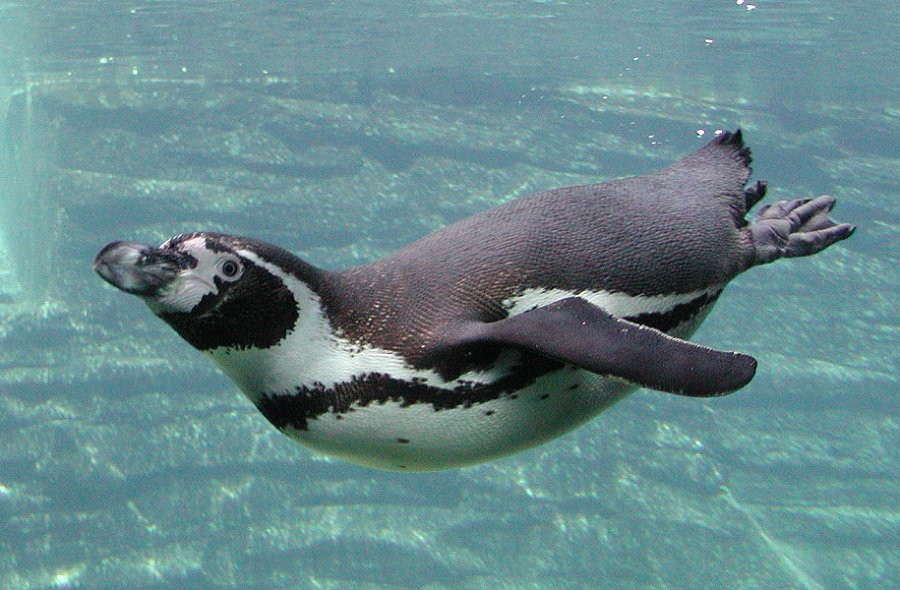
\includegraphics[width=4cm]{bilder/swim-Ping.jpg}
\caption{Ein lebendes Exemplar eines Pinguins}
\label{img:pen}
\end{center}
\end{figure}

\subsection{Erklärung 2}
Es heißt aber auch, da\ss \ ursprünglich der Name 'Pinguin' eine Bezeichnung für den 1844 ausgestorbenen, ebenfalls flugunfähigen Riesenalk der Nordhalbkugel war (siehe Bild \ref{img:auk}).

\begin{figure}[H]
\begin{center}
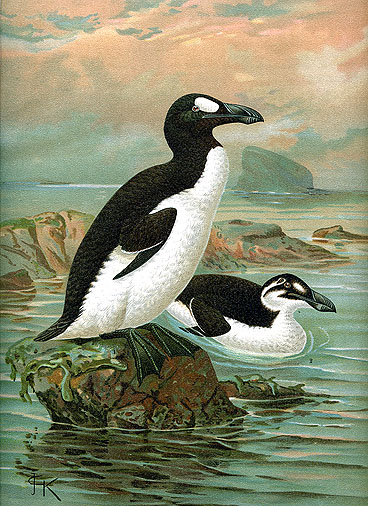
\includegraphics[width=5cm]{bilder/GreatAuk.jpg}
\caption{Ein besonders pr"achtiges Exemplar eines Pinguins}
\label{img:auk}
\end{center}
\end{figure}

\subsection{Erklärung 3}
Eine andere These lautet, dass der Name vom lateinischen "`penguis"' stammt. Dies bedeutet "`Fett"' und für die Seefahrer war Fett sehr wichtig und es ließ sich aus den Pinguinen gewinnen (siehe Bild \ref{img:tux}).

\begin{figure}[H]
\begin{center}

\includegraphics[width=5cm]{bilder/tux.png}
\caption{Der kleine Tux}
\label{img:tux}
\end{center}
\end{figure}

\section{Formeln}
\begin{frame}
\frametitle{Formeln}
\framesubtitle{Mathematische Formeln einbinden}

\begin{exampleblock}{Neue Pakete in diesem Abschnitt}
\begin{multicols}{2}
\begin{itemize}
\item amsmath 
\item amsthm
\item amssymb
\item mathtools
\end{itemize}
\end{multicols}
\end{exampleblock}

\begin{block}{Neue Befehle in diesem Abschnitt}
\begin{multicols}{2}
\begin{itemize}
\item \color{nounibaredI}\textbackslash sqrt\color{black}\{\}
\item \color{nounibaredI}\textbackslash frac\color{black}\{\}\{\}
\item \color{nounibaredI}\textbackslash int\color{black}\_X
\item \color{nounibaredI}\textbackslash sum\color{black}\_\{\}
\item \color{nounibaredI}\textbackslash lim\color{black}\_\{\}
\item \color{nounibaredI}\textbackslash prod\color{black}
\item \color{nounibaredI}\textbackslash limits\color{black}\_\{\}
\item \color{nounibaredI}\textbackslash dots\color{black}
\item \color{nounibaredI}\textbackslash cdot\color{black}
\item \color{nounibaredI}\_\color{black}
\item \color{nounibaredI}\^~\color{black}
\end{itemize}
\end{multicols}
\end{block}

\end{frame}

%-------------------------------------------------------------------------------
\begin{frame}
\frametitle{Formeln}
\framesubtitle{\ldots ~in \LaTeX ~eine wahre Sch\"onheit!}

\begin{columns}
\begin{column}{.3\textwidth}
{\huge $2 \sqrt{\frac{\pi ^2}{3}\cdot c_{2}}$}
\end{column}

\begin{column}{.7\textwidth}
$\underbrace{\color{unibayellowI}\text{\$}%
\color{black}2%
\color{nounibaredI}\backslash \text{sqrt}%
\color{black}\{%
\color{nounibaredI}\backslash \text{frac}%
\color{black}\{%
\color{nounibaredI}\backslash \text{pi}\color{nounibaredI}\^~{}\color{black}2\}\{3\color{black}\}%
\color{nounibaredI}\backslash%
\color{nounibaredI}\text{cdot}~%
\color{black} c%\color{nounibaredI}\_%
\color{black}2\}%
\color{unibayellowI}\$%
}$\color{black}

Die Formel-Umgebung wird durch \color{unibayellowI}\$ \color{black} angefangen und beendet.

\medskip
$\color{unibayellowI}\$\color{black}\underbrace{2\color{nounibaredI}$\color{nounibaredI}\backslash$sqrt\color{black}\{\color{nounibaredI}$\color{nounibaredI}\backslash$frac\color{black}\{\color{nounibaredI}$\color{nounibaredI}\backslash$pi\color{nounibaredI}\^ {}\color{black}2\}\{3\color{black}\}\color{nounibaredI}$\color{nounibaredI}\backslash$cdot~\color{black} c\color{nounibaredI}\_\color{black}2\}$}\color{unibayellowI}\$\color{black} 

So weit reicht die Wurzel.

\bigskip
$\color{unibayellowI}\$\color{black}2\color{nounibaredI}$\color{nounibaredI}\backslash$sqrt\color{black}\underbrace{\{\color{nounibaredI}$\color{nounibaredI}\backslash$frac\color{black}\{\color{nounibaredI}$\color{nounibaredI}\backslash$pi\color{nounibaredI}\^ {}\color{black}2\}\{3\color{black}\}\color{nounibaredI}$}\color{nounibaredI}\backslash$\color{nounibaredI}cdot~\color{black} c\color{nounibaredI}\_\color{black}2\}$\color{unibayellowI}\$\color{black} 

Ein Bruch hat immer Z"ahler und Nenner.
\end{column}
\end{columns}
\end{frame}

%-------------------------------------------------------------------------------

\begin{frame}
\frametitle{Formeln}
\framesubtitle{\ldots ~in \LaTeX ~eine wahre Sch\"onheit!}
\begin{columns}
\begin{column}{.4\textwidth}
\flushright
$\int_0^\infty$
\end{column}
\begin{column}{.6\textwidth}
\flushleft
{\ttfamily\color{unibayellowI}\$\color{nounibaredI}\textbackslash\color{nounibaredI}int\_\color{black}0\color{nounibaredI}\textasciicircum \textbackslash infty\color{unibayellowI}\$}
\end{column}
\end{columns}
\begin{columns}
\begin{column}{.4\textwidth}
\flushright
$\sum_{i=1}^n$
\end{column}
\begin{column}{.6\textwidth}
\flushleft
{\ttfamily $\color{unibayellowI}\$$\color{nounibaredI}\backslash$\color{nounibaredI}sum\_\color{black}\{i=1\}\color{nounibaredI}\^{}\color{black}n\color{unibayellowI}\$}
\end{column}
\end{columns}

\begin{columns}
\begin{column}{.4\textwidth}
\flushright
$\lim_{n \rightarrow \infty}$
\end{column}
\begin{column}{.6\textwidth}
\flushleft
{\ttfamily $\color{unibayellowI}\$$\color{nounibaredI}\backslash$\color{nounibaredI}lim\_\color{black}\{n $\color{nounibaredI}\backslash$\color{nounibaredI}rightarrow $\color{nounibaredI}\backslash$infty\color{black}\}\color{unibayellowI}\$}
\end{column}
\end{columns}

\begin{columns}
\begin{column}{.4\textwidth}
\flushright
$\prod\limits_{i=1}^{n+1}i = 1 \cdot 2 \cdot \ldots \cdot n \cdot (n+1)$
\end{column}
\begin{column}{.6\textwidth}
\flushleft
{\ttfamily $\color{unibayellowI}\$$\color{nounibaredI}\backslash$\color{nounibaredI}prod\textbackslash limits\_\color{black}\{i=1\}\color{nounibaredI}\^{}\color{black}\{n+1\}i = 1 \color{nounibaredI}\backslash$\color{nounibaredI}cdot \color{black}2 \color{nounibaredI}\backslash$\color{nounibaredI}cdot \color{nounibaredI}\backslash$\color{nounibaredI}ldots \color{nounibaredI}\backslash$\color{nounibaredI}cdot \color{black}n \color{nounibaredI}\backslash$\color{nounibaredI}cdot \color{black}(n+1)\color{unibayellowI}\$}
\end{column}
\end{columns}
\bigskip
Die  American Mathematical Society hat einen wundersch"onen Guide f"ur das {\ttfamily amsmath}-Package.\footnote{ftp://ftp.ams.org/pub/tex/doc/amsmath/amsldoc.pdf}
\end{frame}
\section{Code}

\begin{frame}
\frametitle{Code}
\framesubtitle{Programmcode darstellen}

\begin{exampleblock}{Neue Pakete in diesem Abschnitt}
\begin{multicols}{3}
\begin{itemize}
\item verbatim
\item listings
\item color
\end{itemize}
\end{multicols}
\end{exampleblock}

\begin{block}{Neue Befehle in diesem Abschnitt}
%\begin{multicols}{2}
\begin{itemize}
\item \color{nounibaredI}\textbackslash color\color{black}\{\}
\item \color{nounibaredI}\textbackslash lstset\color{black}\{\}
%TODO mehr?
\end{itemize}
%\end{multicols}
\end{block}

\end{frame}

\begin{frame}[fragile]
\frametitle{Code}
\framesubtitle{Unformatierte Texte \& Codeabschnitte}
Die Verbatim Umgebung:\\
\begin{columns}
\begin{column}{.5\textwidth}
\begin{verbatim}
Dieser Satz erscheint
so im Text.
Auch Befehle wie
\textbf{werden}
nicht interpretiert.
\end{verbatim}
\end{column}
\begin{column}{.5\textwidth}
\begin{ttfamily}
\begin{tabbing}
x\=\kill\\
\>\color{unibablueI}\textbackslash begin\color{black}\{verbatim\}\\
\>Dieser Satz erscheint\\
\>so im Text.\\
\>Auch Befehle wie\\
\>\textbackslash textbf\{werden\}\\
\>nicht interpretiert.\\
\>\color{unibablueI}\textbackslash end\color{black}\{verbatim\}\\
\end{tabbing}
\end{ttfamily}
\end{column}
\end{columns}
\end{frame}

%-------------------------------------------------------------------------------

\begin{frame}[fragile]
\frametitle{Code}
\framesubtitle{Unformatierte Texte \& Codeabschnitte}
\vspace{3mm}
%Die Verbatim Umgebung (Paket: verbatim):\\
\scriptsize
\lstset{language=Java, commentstyle=\color{green}}
\begin{lstlisting}
public static void printNumber(int n)
{
    for (int i = 0; i < n; i++)
    {
        // print the current number
        System.out.println("Number: " + i);
    }
}
\end{lstlisting}

\footnotesize
\vspace{-2mm}

\begin{ttfamily}
\begin{tabbing}
xx\=xx\=\kill\\
\color{nounibaredI}\textbackslash usepackage\color{black}\{listings\}\\
\color{nounibaredI}\textbackslash usepackage\color{black}\{color\}\\
\color{nounibaredI}\textbackslash lstset\color{black}\{language=Java, commentstyle=\color{nounibaredI}\textbackslash color\color{black}\{green\}\}\\
\color{unibablueI}\textbackslash begin\color{black}\{lstlisting\}\\
public static void printNumber(int n)\\
\{\\
\>for (int i = 0; i < n; i++)\\
\>\{\\
\>\>// print the current number\\
\>\>System.out.println(\verb|"|Number: \verb|"| + i);\\
\>\}\\
\}\\
\color{unibablueI}\textbackslash end\color{black}\{lstlisting\}\\
\end{tabbing}
\end{ttfamily}
\normalsize
\end{frame}



%TODO hinweis auf weitere Formatierungsmöglichkeiten -> syntax hilighting (siehe Internet)


\section{Tables}

\begin{frame}
\frametitle{Tables}
\framesubtitle{Insertion Of Tables}

\begin{exampleblock}{New packages in this section}
\begin{itemize}
\item longtable
\end{itemize}
\end{exampleblock}

\begin{block}{New commands in this section}
\begin{itemize}
\item \color{unibablueI}\textbackslash begin\color{black}\{tabular\} \dots
~\color{unibablueI}\textbackslash end\color{black}\{tabular\}
\item \color{unibablueI}\textbackslash begin\color{black}\{table\} \dots
~\color{unibablueI}\textbackslash end\color{black}\{table\}
\item \color{unibablueI}\textbackslash begin\color{black}\{longtable\} \dots
~\color{unibablueI}\textbackslash end\color{black}\{longtable\}
\item \color{unibablueI}\textbackslash begin\color{black}\{tabbing\} \dots
~\color{unibablueI}\textbackslash end\color{black}\{tabbing\}
\item \color{nounibaredI}$|$\color{black}
\item \color{nounibaredI}\& \color{black}
\item \color{nounibaredI}\textbackslash hline\color{black}
\item \color{nounibaredI}\textbackslash multicolumn\color{black}\{\}\{\}\{\}
\end{itemize}
\end{block}

\end{frame}

\begin{frame}
\frametitle{Tables}
\framesubtitle{``table'' \& \glqq tabular\grqq}
\textbf{Structure:}\\[2mm]
\color{unibablueI}\begin{ttfamily}\textbackslash begin\color{black}\{table\}\color{nounibagreenI}[position]\color{black}\\
\color{unibablueI}\textbackslash begin\color{black}\{tabular\}\{\textit{Definition of columns}\}\\
\textit{Table content}\\
\color{unibablueI}\textbackslash end\color{black}\{tabular\}\\
\color{nounibaredI}\textbackslash caption\color{black}\{caption\}\\
\color{nounibaredI}\textbackslash label\color{black}\{tab:bsptab1\}\\
\color{unibablueI}\textbackslash end\color{black}\{table\}\\
~\\
\end{ttfamily}

\begin{block}{Reminder: positioning in most \LaTeX -- environments}
\color{nounibagreenI}[h]\color{black}~or \color{nounibagreenI}[H]\color{black}~= At this very position\\
\color{nounibagreenI}[t]\color{black}~= On top of the page\\ 
\color{nounibagreenI}[b]\color{black}~= On bottom of the page\\ 
\color{nounibagreenI}[p]\color{black}~= Positioning on an own page
\end{block}
\end{frame}


\begin{frame}
\frametitle{Tables}
\framesubtitle{Definition Of Columns}
Here you can define how the columns should be aligned
and how the vertical lines should be set:\\[3mm]
\begin{tabbing}[H]p{column width}xxx\=\kill
\textbf{Commands:}\\
l \>= left-justified\\
c \>= centered\\
r \>= right-justified\\
p\{column width\} \>= a left-justified column with defined width\\
\color{nounibaredI}$|$\color{black} \>= sets a vertical line
at this position\\
\end{tabbing}
\end{frame}

\begin{frame}
\frametitle{Tables}
\framesubtitle{View From Inside}
\begin{ttfamily}
\color{nounibaredI}\color{unibablueI}\textbackslash\color{unibablueI}begin\color{black}\color{black}\{tabular\}\{c\color{nounibaredI}|\color{black}p\{40mm\}\color{nounibaredI}|\color{black}lr\color{nounibaredI}|\color{black}c\} \\
\color{nounibaredI}\color{nounibaredI}\textbackslash multicolumn\color{black}\{5\}\{c\}\{E-Sports Championship Franconia\} \color{nounibaredI}\color{nounibaredI}\textbackslash \color{nounibaredI}\textbackslash \color{black} \\
\color{nounibaredI}\color{nounibaredI}\textbackslash hline\color{black} \\
\color{nounibaredI}\color{nounibaredI}\textbackslash hline\color{black} \\
Number \color{nounibaredI}\&  \color{black}Place \color{nounibaredI}\&  \color{black}Player 1 \color{nounibaredI}\&  \color{black}Player 2 \color{nounibaredI}\&  \color{black}Result \color{nounibaredI}\color{nounibaredI}\textbackslash \color{nounibaredI}\textbackslash \color{black} \\
\color{nounibaredI}\color{nounibaredI}\textbackslash hline\color{black} \\
1 \color{nounibaredI}\&  \color{black}Nürnberg \color{nounibaredI}\&  \color{black}Wolf \color{nounibaredI}\&  \color{black}Lamm \color{nounibaredI}\&  \color{black}23:10 \color{nounibaredI}\color{nounibaredI}\textbackslash \color{nounibaredI}\textbackslash \color{black} \\
\color{nounibaredI}\color{nounibaredI}\textbackslash hline\color{black} \\
2 \color{nounibaredI}\&  \color{black}Bamberg \color{nounibaredI}\&  \color{black}Meyer \color{nounibaredI}\&  \color{black}Beyer \color{nounibaredI}\color{nounibaredI}\textbackslash \color{nounibaredI}\textbackslash \color{black} \\
\color{nounibaredI}\color{nounibaredI}\textbackslash hline\color{black} \\
3 \color{nounibaredI}\&  \color{black}Zirndorf \color{nounibaredI}\&  \color{black}Brandst. \color{nounibaredI}\&  \color{black}Brauer \color{nounibaredI}\&  \color{black}21:21\color{nounibaredI}\color{nounibaredI}\textbackslash \color{nounibaredI}\textbackslash \color{black} \\
\color{nounibaredI}\color{nounibaredI}\textbackslash hline\color{black} \\
\color{nounibaredI}\color{unibablueI}\textbackslash\color{unibablueI}end\color{black}\color{black}\{tabular\} \\

\end{ttfamily}
\end{frame}

\begin{frame}
\frametitle{Tables}
\framesubtitle{Table Content}
Here you fill the defined columns with content.\\[3mm]
\begin{tabbing}[H]p{column width}xxx\=\kill
\textbf{Commands:}\\
\color{nounibaredI}\&\color{black} \>= horizontal separation of rows\\
\color{nounibaredI}\textbackslash \textbackslash \color{black} \>=  new line\\
\color{nounibaredI}\textbackslash hline\color{black} \>= sets a horizontal line\\[2mm]
\color{nounibaredI}\textbackslash multicolumn\color{black}\{column number\}\{column alignment\}\{text\}\\[2mm]
\>= Combines as many columns as you like.\\
\end{tabbing}
\end{frame}

\begin{frame}[t]

\frametitle{Tables}
\framesubtitle{Example Tabular}
\begin{footnotesize}
\begin{ttfamily}
\color{nounibaredI}\color{unibablueI}\textbackslash\color{unibablueI}begin\color{black}\color{black}\{tabular\}\{c\color{nounibaredI}|\color{black}p\{40mm\}\color{nounibaredI}|\color{black}lr\color{nounibaredI}|\color{black}c\} \\
\color{nounibaredI}\color{nounibaredI}\textbackslash multicolumn\color{black}\{5\}\{c\}\{E-Sports Championship Franconia\} \color{nounibaredI}\color{nounibaredI}\textbackslash \color{nounibaredI}\textbackslash \color{black} \\
\color{nounibaredI}\color{nounibaredI}\textbackslash hline\color{black} \\
\color{nounibaredI}\color{nounibaredI}\textbackslash hline\color{black} \\
Number \color{nounibaredI}\&  \color{black}Place \color{nounibaredI}\&  \color{black}Player 1 \color{nounibaredI}\&  \color{black}Player 2 \color{nounibaredI}\&  \color{black}Result \color{nounibaredI}\color{nounibaredI}\textbackslash \color{nounibaredI}\textbackslash \color{black} \\
\color{nounibaredI}\color{nounibaredI}\textbackslash hline\color{black} \\
1 \color{nounibaredI}\&  \color{black}Nürnberg \color{nounibaredI}\&  \color{black}Wolf \color{nounibaredI}\&  \color{black}Lamm \color{nounibaredI}\&  \color{black}23:10 \color{nounibaredI}\color{nounibaredI}\textbackslash \color{nounibaredI}\textbackslash \color{black} \\
\color{nounibaredI}\color{nounibaredI}\textbackslash hline\color{black} \\
2 \color{nounibaredI}\&  \color{black}Bamberg \color{nounibaredI}\&  \color{black}Meyer \color{nounibaredI}\&  \color{black}Beyer \color{nounibaredI}\color{nounibaredI}\textbackslash \color{nounibaredI}\textbackslash \color{black} \\
\color{nounibaredI}\color{nounibaredI}\textbackslash hline\color{black} \\
3 \color{nounibaredI}\&  \color{black}Zirndorf \color{nounibaredI}\&  \color{black}Brandst. \color{nounibaredI}\&  \color{black}Brauer \color{nounibaredI}\&  \color{black}21:21\color{nounibaredI}\color{nounibaredI}\textbackslash \color{nounibaredI}\textbackslash \color{black} \\
\color{nounibaredI}\color{nounibaredI}\textbackslash hline\color{black} \\
\color{nounibaredI}\color{unibablueI}\textbackslash\color{unibablueI}end\color{black}\color{black}\{tabular\} \\

\end{ttfamily}
\end{footnotesize}

\begin{tabular}{c|p{40mm}|lr|c}
\multicolumn{5}{c}{E-Sports Championship Franconia}
 \\
\hline
\hline
Number & Place & Player 1 & Player 2 & Result \\
\hline
1 & N\"urnberg & Wolf & Lamm & 23:10 \\
\hline
2 & Bamberg & Meyer & Beyer & \\
\hline
3 & Zirndorf & Brandst. & Brauer & 21:21 \\
\hline
\end{tabular}
\end{frame}

\begin{frame}{Tables}
\framesubtitle{Longtable -- Table With Line Break}
\bigskip
„tabular“ shows the table on one page. If it does not fit on the page, the remainder is cut off.\\
For tables longer than one page, a table is needed that performs a division of the table.\\
\textbf{Solution: {\ttfamily longtable}}\\
{\ttfamily longtable} allows a line break in the table. Moreover, {\ttfamily longtable} is an environment, so the  {\ttfamily table}-environment is not needed anymore!\\[3mm]

\begin{ttfamily}
\color{unibablueI}\textbackslash begin\color{black}\{longtable\}\{\textit{definition of columns}\}\\
\textit{table content}\\
\color{nounibaredI}\textbackslash caption\color{black}\{caption\}\\
\color{nounibaredI}\textbackslash label\color{black}\{tab:bsptab2\}\\
\color{unibablueI}\textbackslash end\color{black}\{longtable\}
\end{ttfamily}
\end{frame}


\begin{frame}
\frametitle{Indentations With „tabbing“}
\begin{block}{Control}
\begin{itemize}
\item[\begin{ttfamily}\color{nounibaredI}\textbackslash =\end{ttfamily}]\color{black}set a tab position 
\item[\begin{ttfamily}\color{nounibaredI}\textbackslash $>$\end{ttfamily}]select a tab position
\end{itemize}
\end{block}

\begin{columns}
\begin{column}{.5\textwidth}
\begin{ttfamily}{\scriptsize
\color{nounibaredI}\color{nounibaredI}\textbackslash documentclass\color{black}\{article\} \\
\color{nounibaredI}\color{unibablueI}\textbackslash\color{unibablueI}begin\color{black}\color{black}\{document\} \\
\color{nounibaredI}\color{unibablueI}\textbackslash\color{unibablueI}begin\color{black}\color{black}\{tabbing\} \\
Employ\color{nounibaredI}\color{nounibaredI}\textbackslash \color{black}=ee:\color{nounibaredI}\color{nounibaredI}\textbackslash \color{nounibaredI}\textbackslash \color{black} \\
A  \color{nounibaredI}\color{nounibaredI}\textbackslash \color{black}> Daniel\color{nounibaredI}\color{nounibaredI}\textbackslash \color{nounibaredI}\textbackslash \color{black} \\
B  \color{nounibaredI}\color{nounibaredI}\textbackslash \color{black}> Martin\color{nounibaredI}\color{nounibaredI}\textbackslash \color{nounibaredI}\textbackslash \color{black} \\
C  \color{nounibaredI}\color{nounibaredI}\textbackslash \color{black}> Linus\color{nounibaredI}\color{nounibaredI}\textbackslash \color{nounibaredI}\textbackslash \color{black} \\
xxx\color{nounibaredI}\color{nounibaredI}\textbackslash \color{black}=xxx\color{nounibaredI}\color{nounibaredI}\textbackslash \color{black}=xxxxxxx\color{nounibaredI}\color{nounibaredI}\textbackslash kill\color{black} \\
\color{nounibaredI}\color{nounibaredI}\textbackslash \color{black}> Committees\color{nounibaredI}\color{nounibaredI}\textbackslash \color{nounibaredI}\textbackslash \color{black} \\
\color{nounibaredI}\color{nounibaredI}\textbackslash \color{black}>\color{nounibaredI}\color{nounibaredI}\textbackslash \color{black}> Tests\color{nounibaredI}\color{nounibaredI}\textbackslash \color{nounibaredI}\textbackslash \color{black} \\
\color{nounibaredI}\color{nounibaredI}\textbackslash \color{black}>\color{nounibaredI}\color{nounibaredI}\textbackslash \color{black}> Mails\color{nounibaredI}\color{nounibaredI}\textbackslash \color{nounibaredI}\textbackslash \color{black} \\
\color{nounibaredI}\color{unibablueI}\textbackslash\color{unibablueI}end\color{black}\color{black}\{tabbing\} \\
\color{nounibaredI}\color{unibablueI}\textbackslash\color{unibablueI}end\color{black}\color{black}\{document\} \\
}
\end{ttfamily}
\end{column}
\begin{column}{.5\textwidth}
\begin{tabbing}
Employ\=ee:\\
A  \> Daniel\\
B  \> Martin\\
C  \> Linus\\
xxx\=xxx\=xxxxxxx\kill
\> Committees\\
\>\> Tests\\
\>\> Mails\\
\end{tabbing}
\end{column}
\end{columns}

If you use the command \begin{ttfamily}\color{nounibaredI}\textbackslash kill\color{black}\end{ttfamily}, the rest of the line is not shown. In this way you can do the formatting without showing the respective text.
\end{frame}

\section{Aufz\"ahlungen}
\begin{frame}
\frametitle{Aufzählungen}

\begin{block}{Neue Befehle in diesem Abschnitt}
\begin{itemize}
\item \color{unibablueI}\textbackslash begin\color{black}\{itemize\} \ldots \color{unibablueI}\textbackslash end\color{black}\{itemize\} 
\item \color{unibablueI}\textbackslash begin\color{black}\{enumerate\} \ldots \color{unibablueI}\textbackslash end\color{black}\{enumerate\} 
\item \color{nounibaredI}\textbackslash item\color{black}
\end{itemize}
\end{block}
\end{frame}

\begin{frame}
\frametitle{Aufzählungen}
\framesubtitle{Spiegelstrichlisten}

\begin{columns}
\begin{column}{.5\textwidth}
\begin{ttfamily}
\color{nounibaredI}\color{nounibaredI}\textbackslash documentclass\color{black}\{article\} \\
\color{nounibaredI}\color{unibablueI}\textbackslash\color{unibablueI}begin\color{black}\color{black}\{document\} \\
\color{nounibaredI}\color{unibablueI}\textbackslash\color{unibablueI}begin\color{black}\color{black}\{itemize\} \\
\color{nounibaredI}\color{nounibaredI}\textbackslash item\color{black} erster Stichpunkt \\
\color{nounibaredI}\color{nounibaredI}\textbackslash item\color{black} zweiter Stichpunkt \\
\color{nounibaredI}\color{nounibaredI}\textbackslash item\color{black} dritter Stichpunkt \\
\color{nounibaredI}\color{nounibaredI}\textbackslash item\color{black} letzter Stichpunkt \\
\color{nounibaredI}\color{unibablueI}\textbackslash\color{unibablueI}end\color{black}\color{black}\{itemize\} \\
\color{nounibaredI}\color{unibablueI}\textbackslash\color{unibablueI}end\color{black}\color{black}\{document\} \\
\end{ttfamily}
\end{column}
\begin{column}{.5\textwidth}
\begin{itemize}
\item erster Stichpunkt
\item zweiter Stichpunkt
\item dritter Stichpunkt
\item letzter Stichpunkt
\end{itemize}
\end{column}
\end{columns}
\bigskip

Die einzelnen Stichpunkte werden innerhalb der „itemize“-Umgebung durch den Befehl \begin{ttfamily}\color{nounibaredI}\textbackslash item\color{black}\end{ttfamily} gekennzeichnet.
\end{frame}

\begin{frame}
\frametitle{Aufzählungen}
\framesubtitle{Verschachtelung}

\begin{columns}
\begin{column}{.5\textwidth}
\begin{ttfamily}
\color{nounibaredI}\color{nounibaredI}\textbackslash documentclass\color{black}\{article\} \\
\color{nounibaredI}\color{unibablueI}\textbackslash\color{unibablueI}begin\color{black}\color{black}\{document\} \\
\color{nounibaredI}\color{unibablueI}\textbackslash\color{unibablueI}begin\color{black}\color{black}\{itemize\} \\
\color{nounibaredI}\color{nounibaredI}\textbackslash item \color{black} erster Stichpunkt \\
\color{nounibaredI}\color{nounibaredI}\textbackslash item \color{black} zweiter Stichpunkt \\
\color{nounibaredI}\color{unibablueI}\textbackslash\color{unibablueI}begin\color{black}\color{black}\{itemize\} \\
\color{nounibaredI}\color{nounibaredI}\textbackslash item \color{black} erster Unterpunkt \\
\color{nounibaredI}\color{nounibaredI}\textbackslash item \color{black} zweiter Unterpunkt \\
\color{nounibaredI}\color{unibablueI}\textbackslash\color{unibablueI}end\color{black}\color{black}\{itemize\} \\
\color{nounibaredI}\color{nounibaredI}\textbackslash item \color{black} dritter Stichpunkt \\
\color{nounibaredI}\color{nounibaredI}\textbackslash item \color{black} letzter Stichpunkt \\
\color{nounibaredI}\color{unibablueI}\textbackslash\color{unibablueI}end\color{black}\color{black}\{itemize\} \\
\color{nounibaredI}\color{unibablueI}\textbackslash\color{unibablueI}end\color{black}\color{black}\{document\} \\
\end{ttfamily}
\end{column}
\begin{column}{.5\textwidth}
\begin{itemize}
\item erster Stichpunkt
\item zweiter Stichpunkt
\begin{itemize}
\item erster Unterpunkt
\item zweiter Unterpunkt
\end{itemize}
\item dritter Stichpunkt
\item letzter Stichpunkt
\end{itemize}
\end{column}
\end{columns}
\bigskip
Auf diese Weise kann man Unterpunkte bis auf 4 Ebenen tief schachteln.
\end{frame}


\begin{frame}
\frametitle{Aufzählungen}
\framesubtitle{Nummerierungen}

\begin{columns}
\begin{column}{.5\textwidth}
\begin{ttfamily}
\color{nounibaredI}\color{nounibaredI}\textbackslash documentclass\color{black}\{article\} \\
\color{nounibaredI}\color{unibablueI}\textbackslash\color{unibablueI}begin\color{black}\color{black}\{document\} \\
\color{nounibaredI}\color{unibablueI}\textbackslash\color{unibablueI}begin\color{black}\color{black}\{enumerate\} \\
\color{nounibaredI}\color{nounibaredI}\textbackslash item \color{black} first bullet item \\
\color{nounibaredI}\color{unibablueI}\textbackslash\color{unibablueI}begin\color{black}\color{black}\{enumerate\} \\
\color{nounibaredI}\color{nounibaredI}\textbackslash item \color{black} first subitem \\
\color{nounibaredI}\color{nounibaredI}\textbackslash item \color{black} second subitem \\
\color{nounibaredI}\color{unibablueI}\textbackslash\color{unibablueI}end\color{black}\color{black}\{enumerate\} \\
\color{nounibaredI}\color{nounibaredI}\textbackslash item \color{black} second bullet item \\
\color{nounibaredI}\color{nounibaredI}\textbackslash item \color{black} and so forth \\
\color{nounibaredI}\color{unibablueI}\textbackslash\color{unibablueI}end\color{black}\color{black}\{enumerate\} \\
\color{nounibaredI}\color{unibablueI}\textbackslash\color{unibablueI}end\color{black}\color{black}\{document\} \\
\end{ttfamily}
\end{column}
\begin{column}{.5\textwidth}
\begin{enumerate}
\item erstens
\begin{enumerate}
\item erster Unterpunkt
\item zweiter Unterpunkt
\end{enumerate}
\item zweitens
\item usw.
\end{enumerate}
\end{column}
\end{columns}
\bigskip
Auch hier werden die einzelnen Punkte durch den Befehl \begin{ttfamily}\color{nounibaredI}\textbackslash item\color{black}\end{ttfamily} gekennzeichnet. 
Schachtelungen können wieder bis zu 4 Ebenen tief sein.
\end{frame}

\begin{frame}
\frametitle{Gemischte Aufzählungen?}
\framesubtitle{Geht Alles!}

\begin{columns}
\begin{column}{.5\textwidth}
\begin{ttfamily}
\color{nounibaredI}\color{unibablueI}\textbackslash\color{unibablueI}begin\color{black}\color{black}\{enumerate\} \\
\color{nounibaredI}\color{nounibaredI}\textbackslash item\color{black} erstens \\
\color{nounibaredI}\color{nounibaredI}\textbackslash item\color{black} \color{nounibaredI}\color{unibablueI}\textbackslash\color{unibablueI}begin\color{black}\color{black}\{itemize\} \\
\color{nounibaredI}\color{nounibaredI}\textbackslash item\color{black} erster Unterpunkt \\
\color{nounibaredI}\color{nounibaredI}\textbackslash item\color{black} zweiter Unterpunkt \\
\color{nounibaredI}\color{unibablueI}\textbackslash\color{unibablueI}end\color{black}\color{black}\{itemize\} \\
\color{nounibaredI}\color{nounibaredI}\textbackslash item\color{black} drittens \\
\color{nounibaredI}\color{unibablueI}\textbackslash\color{unibablueI}begin\color{black}\color{black}\{enumerate\} \\
\color{nounibaredI}\color{nounibaredI}\textbackslash item\color{black} Auch ich zähle! \\
\color{nounibaredI}\color{unibablueI}\textbackslash\color{unibablueI}end\color{black}\color{black}\{enumerate\} \\
\color{nounibaredI}\color{nounibaredI}\textbackslash item\color{black} usw. \\
\color{nounibaredI}\color{unibablueI}\textbackslash\color{unibablueI}end\color{black}\color{black}\{enumerate\} \\
\end{ttfamily}
\end{column}
\begin{column}{.5\textwidth}
\begin{enumerate}
\item erstens
\item \begin{itemize}
\item erster Unterpunkt
\item zweiter Unterpunkt
\end{itemize}
\item drittens
\begin{enumerate}
\item Auch ich z"ahle!
\end{enumerate}
\item usw.
\end{enumerate}
\end{column}
\end{columns}
\bigskip
Die Darstellung der jeweiligen Symbole kann mit \color{nounibaredI}\textbackslash item\color{nounibagreenI}[]\color{black}~angepasst werden. 
\end{frame}
\documentclass[a4paper, pdftex, ngerman, 11pt]{article}
%IMMER!!!
\usepackage[utf8]{inputenc}
\usepackage[T1]{fontenc}
\usepackage{babel}
\usepackage[iso]{umlaute}

\usepackage{longtable}
\usepackage{listings}
\usepackage{color}

\begin{document}
\section{Aufgabe 4}
\subsection{Tabellen \& Formeln}
Die Tabelle \ref{tab:ani} besteht aus 3 Spalten:\\
Die erste Spalte ist mit einem p von 25mm definiert. Die zweite und die dritte Spalte sind zentriert.

\begin{longtable}{p{25mm}|c|c}
& Fuchs & Elster\\
\hline
\hline
Familie & Hunde & Rabenvögel\\
\hline
Gewicht & m: 6,6kg w: 5,5kg & 200--250g\\
\hline
Geschwindigkeit $ = \sqrt{v\cdot v}$ & $55\frac{km}{h}$ & mind. superschnell: $\lim\limits_{x \rightarrow \infty} x \cdot v$ \\
\hline
Farbe & tödlich & schwarz\\
\hline
\caption{Wild Animals}
\label{tab:ani}
\end{longtable}

Der Sinn des Lebens$^2$: $\prod\limits_{i=1}^{n+1} i + \sum_{j=0}^{n} j \cdot \int\limits_{\pi}^{Daumen} 42$

\subsection{Aufzählungen}
Um bei den vielen Verschachtelungen nicht den Überblick zu verlieren, sind Einrückungen der items sinnvoll.
\begin{enumerate}
  \item 
  \begin{enumerate}
    \item Vorteile des Fuchses:
    \item
    \begin{itemize}
      \item schlau
      \item schaut cool aus
    \end{itemize}
    \item Nachteile des Fuchses:
    \begin{itemize}
      \item Pelz wird verarbeitet
      \item sehr viele Autos fahren gerne über Füchse
    \end{itemize}
    \item Spam Spam Spam
  \end{enumerate}
  \item
  \begin{enumerate}
    \item Vorteile der Elster...
    \item Nachteile der Elster:
    \begin{itemize}
      \item Diebischkeit wird bestraft
      \item viele landen hinter Gittern
    \end{itemize}
      \item singt ganz gut, aber ist gefährlich
  \end{enumerate}
\end{enumerate}

\subsection{(Un)Logik}
\begin{itemize}
	\item $\lnot\forall x \Leftrightarrow \{\exists x\}$
	\item $[\exists xPx] \rightarrow \forall x \lnot Px$
\end{itemize}

\subsection{Code}
\textit{Hello World} in Java:\\
\lstset{language=Java, commentstyle=\color{green}}
\begin{lstlisting}
  public class Hello{
      public static void main(String[] args){
      
         //Hier wird der Text ausgegeben:
         System.out.println("Hello World!");
      }
  }
\end{lstlisting}

\end{document}
\section{Vert. Arbeiten}
\begin{frame}
\frametitle{Ein handfestes Dokument aufbauen}
\framesubtitle{\ldots und dabei den vollen Charme von \LaTeX ~erleben!}
\begin{block}{Neue Befehle in diesem Abschnitt}
\begin{itemize}
  \item \color{nounibaredI}\textbackslash input\color{black}\{\}
  \item \color{nounibaredI}\textbackslash tableofcontents\color{black}
  \item \color{nounibaredI}\textbackslash listoffigures\color{black}
  \item \color{nounibaredI}\textbackslash listoftables\color{black}
  \item \color{nounibaredI}\textbackslash vspace\color{black}\{\}
  \item \color{nounibaredI}\textbackslash today\color{black}
\item \color{unibablueI}\textbackslash begin\color{black}\{titlepage\} \ldots \color{unibablueI}\textbackslash end\color{black}\{titlepage\} 
\end{itemize}
\end{block}
\end{frame}

%-----------------------------------------------------------------------------------------

\begin{frame}
\frametitle{Aufbau von einem gr\"o\ss erem Dokument}

\begin{columns}
\begin{column}{.5\textwidth}
\footnotesize
\begin{figure}[t]
\begin{tikzpicture}[dirtree]
\node {main.tex} 
        child {node {command.tex}}
        child {node {titlepage.tex}}
        %child {node {introduction.tex}}
        child {node {aufgabe1.tex}}
        child {node {aufgabe2.tex}}
        child {node {aufgabe3.tex}}
        %child {node {conclusion.tex}} 
        ;
        %TODO evtl doch wieder einkommentieren?
\end{tikzpicture}
\end{figure}
\end{column}
\begin{column}{.5\textwidth}
In der Hauptdatei (main.tex) werden alle anderen Dateien zu einem Dokument zusammengefasst. 
Dazu muss man die einzelnen Dateien daf\"ur anpassen.
\end{column}
\end{columns}
\end{frame}

%-----------------------------------------------------------------------------------------

\begin{frame}
\frametitle{\ldots ~und das wollen wir nun machen:}
Es muss \textbf{alles} (einschliesslich) vor und nach \color{unibablueI}\textbackslash begin\color{black}- 
und\color{unibablueI}~\textbackslash end\color{black}\{document\} gel\"oscht werden:\\[5mm]
\begin{columns}
\begin{column}{.47\textwidth}
\sout{\color{nounibaredI}\color{nounibaredI}\textbackslash documentclass\color{black}\color{nounibagreenI}[pdftex]\color{black}\{article\} \\
\color{nounibaredI}\textbackslash usepackage\color{black}\{babel\}\\
\color{nounibaredI}\color{unibablueI}\textbackslash\color{unibablueI}begin\color{black}\color{black}\{document\} }\\
Dieses Dokument kann nun mit dem Befehl \color{nounibaredI}\color{nounibaredI}\textbackslash input\color{nounibaredI}\color{black}\{Dateiname\} in LaTeX eingebunden werden.\color{nounibaredI}\color{nounibaredI}\textbackslash \color{nounibaredI}\textbackslash \color{black}  \\
\sout{\color{nounibaredI}\color{unibablueI}\textbackslash\color{unibablueI}end\color{black}\color{black}\{document\} }
\end{column}
\begin{column}{.47\textwidth}
Mit dem Befehl \color{nounibaredI}\textbackslash input\color{black}\{pfad/zur/datei\} kann man danach
 diese in eine andere {\ttfamily .tex}-Datei einbinden.

\end{column}
\end{columns}
\end{frame}

%-----------------------------------------------------------------------------------------

\begin{frame}
\frametitle{Verteiltes Arbeiten}
\framesubtitle{\ldots den \"Uberblick behalten}
\begin{columns}{2}
\begin{column}{.6\textwidth}
\image{\textwidth}{image/outline.png}{Texmaker listet die {\ttfamily\color{nounibaredI}\textbackslash input}\color{black}s}{img:outline}
\end{column}
\begin{column}{.3\textwidth}
\begin{alertblock}{Achtung:}
Die Pfadangabe ist immer relativ zur Hauptdatei!
\end{alertblock}
\end{column}
\end{columns}

\end{frame}


%-----------------------------------------------------------------------------------------

\begin{frame}
\frametitle{Verzeichnisse}
\framesubtitle{Inhaltsverzeichnis, Abbildungsverzeichnis, Tabellenverzeichnis}
\begin{itemize}


\item Inhaltsverzeichnis (Nach dem Deckblatt)\\
\medskip
\begin{ttfamily}{\normalsize
\color{nounibaredI}\textbackslash tableofcontents\\}
\end{ttfamily}
\medskip
In das Inhaltsverzeichnis werden alle Gliderungspunkte (u.a. \color{unibablueI} \textbackslash section\color{black}s) übernommen.\\
\medskip
%\begin{ttfamily}{\normalsize
%\color{unibablueI} \textbackslash chapter\color{black}\{Formeln\}\\
%\color{unibablueI} \textbackslash section\color{black}\{Kategorie ganz einfach\}\\
%\color{unibablueI} \textbackslash subsection\color{black}\{Kategorie geschenkt\}\\
%\color{unibablueI} \textbackslash subsection\color{black}\{Kategorie weichspüler\}\\
%\color{unibablueI} \textbackslash section\color{black}\{Kategorie mittel\}\\
%\color{unibablueI} \textbackslash section\color{black}\{Kategorie hart\}\\
%\color{unibablueI} \textbackslash section\color{black}\{Kategorie ultra\}\\}
%\end{ttfamily}

\item Abbildungsverzeichnis\\
\medskip
\begin{ttfamily}{\normalsize
\color{nounibaredI}\textbackslash listoffigures\\}
\end{ttfamily}
\medskip
Verwendet jeweils den in der {\ttfamily \color{nounibaredI}\textbackslash caption\color{black}\{...\}} des Bildes angegebenen Titel. 
Andere Titel mit:\\ 
\begin{ttfamily}{\normalsize
\color{nounibaredI} \textbackslash caption\color{nounibagreenI}[\textit{Titel für das Verzeichnis}]\color{black}\{\textit{Anderer Titel}\}\\}
\end{ttfamily}
\medskip

\item Tabellenverzeichnis\\
\medskip
\begin{ttfamily}{\normalsize
\color{nounibaredI}\textbackslash listoftables\\}
\end{ttfamily}
\medskip
Vorgehensweise wie beim Abbildungsverzeichnis\\

\end{itemize}
\end{frame}

%-----------------------------------------------------------------------------------------

%\begin{frame}
%\frametitle{Abbildungsverzeichnis}
%Das Abbildungsverzeichnis.\\
%\medskip
%\begin{ttfamily}{\normalsize
%\color{nounibaredI}\textbackslash listoffigures\\}
%\end{ttfamily}
%\medskip
%\textbf{Beachte:}\\
%Dabei wird als Titel für die Grafiken im Abbildungsverzeichnis jeweils der im Befehl {\ttfamily \color{nounibaredI}\textbackslash caption\color{black}\{...\}} angegebene Titel verwendet. Möchte man im Verzeichnis andere Überschriften verwenden, so kann dem {\ttfamily \color{nounibaredI}\textbackslash caption\color{black}}-Befehl dazu ein weiterer Parameter beigefügt werden:\\
%\medskip
%\begin{ttfamily}{\normalsize
%\color{nounibaredI} \textbackslash caption\color{nounibagreenI}[\textit{Titel für das Verzeichnis}]\color{black}\{\textit{Anderer Titel}\}\\}
%\end{ttfamily}
%\end{frame}

%-----------------------------------------------------------------------------------------

%\begin{frame}
%\frametitle{Tabellenverzeichnis}
%Das Tabellenverzeichnis.\\
%\medskip
%\begin{ttfamily}{\normalsize
%\color{nounibaredI}\textbackslash listoftables\\}
%\end{ttfamily}
%\medskip
%\textbf{Beachte:}\\
%Vorgehensweise wie beim Abbildungsverzeichnis:\\
%\medskip
%\textbf{Hinweis:}\\
%Es ist möglich Abbildungen ins Tabellenverzeichnis aufzunehmen und umgekehrt. Dazu die Abbildung einfach in eine  {\ttfamily \color{unibablueI}table\color{black}}-Umgebung packen bzw. die Tabelle in eine {\ttfamily \color{unibablueI}figure\color{black}}-Umgebung.\\
%\end{frame}

%-----------------------------------------------------------------------------------------



\begin{frame}[t]
\frametitle{Exkurs: Titelseite}
\begin{columns}
\begin{column}{0.5\textwidth}
%\begin{titlepage}
\begin{center}
\Huge \LaTeX\\
\vspace{5mm} \LARGE Eine kurze Einführung\\
\vspace{12mm} \Large  Universität Bamberg\\[5mm]
\large 08. April 2015\\
Fachschaft WIAI\normalsize \\
\end{center}
%\end{titlepage}
\end{column}
\begin{column}{0.5\textwidth}
\color{nounibaredI}\color{unibablueI}\textbackslash\color{unibablueI}begin\color{black}\color{black}\{titlepage\} \\\color{black}
\color{nounibaredI}\color{unibablueI}\textbackslash\color{unibablueI}begin\color{black}\color{black}\{center\} \\
\color{nounibaredI}\color{nounibaredI}\textbackslash Huge\color{black} \color{nounibaredI}\color{nounibaredI}\textbackslash LaTeX\color{nounibaredI}\textbackslash \color{nounibaredI}\textbackslash \color{black} \\
\color{nounibaredI}\color{nounibaredI}\textbackslash vspace\color{black}\{5mm\} \color{nounibaredI}\color{nounibaredI}\textbackslash LARGE \color{black} Eine kurze Einführung\color{nounibaredI}\color{nounibaredI}\textbackslash \color{nounibaredI}\textbackslash \color{black} \\
\color{nounibaredI}\color{nounibaredI}\textbackslash vspace\color{black}\{12mm\} \color{nounibaredI}\color{nounibaredI}\textbackslash Large \color{black} Universität Bamberg\color{nounibaredI}\color{nounibaredI}\textbackslash \color{nounibaredI}\textbackslash \color{black}\color{nounibagreenI}[5mm]\color{black} \\
\color{nounibaredI}\color{nounibaredI}\textbackslash large\color{black} \color{nounibaredI}\color{nounibaredI}\textbackslash today\color{nounibaredI}\textbackslash \color{nounibaredI}\textbackslash \color{black} \\
Fachschaft WIAI\color{nounibaredI}\color{nounibaredI}\textbackslash normalsize\color{black} \color{nounibaredI}\color{nounibaredI}\textbackslash \color{nounibaredI}\textbackslash \color{black} \\
\color{nounibaredI}\color{unibablueI}\textbackslash\color{unibablueI}end\color{black}\color{black}\{center\} \\
\color{nounibaredI}\color{unibablueI}\textbackslash\color{unibablueI}end\color{black}\color{black}\{titlepage\} \\\color{black}
\end{column}
\end{columns}
\end{frame}


%-----------------------------------------------------------------------------------------


\begin{frame}
\frametitle{Verteiltes Arbeiten}
\framesubtitle{Beispiel}

\color{nounibaredI}\color{nounibaredI}\textbackslash input\color{black}\{command.tex\} \color{unibagrayI}\% e.g. documentclass, usepackage, usw. auslagern \\\color{black}
\color{nounibaredI}\color{unibablueI}\textbackslash\color{unibablueI}begin\color{black}\color{black}\{document\} \\
\color{nounibaredI}\color{nounibaredI}\textbackslash input\color{black}\{titlepage.tex\} \\
\color{nounibaredI}\color{nounibaredI}\textbackslash tableofcontents\color{black} \\
\color{unibagrayI}\% Jeweils neue Seite \\\color{black}
\color{nounibaredI}\color{nounibaredI}\textbackslash listoffigures\color{black} \\
\color{nounibaredI}\color{nounibaredI}\textbackslash listoftables\color{black} \\
\color{nounibaredI}\color{nounibaredI}\textbackslash input\color{black}\{aufgabe1.tex\} \\
\color{nounibaredI}\color{nounibaredI}\textbackslash input\color{black}\{aufgabe2.tex\} \\
\color{nounibaredI}\color{nounibaredI}\textbackslash input\color{black}\{aufgabe3.tex\} \\
\color{unibagrayI}\% Conclusion, Literature ... \\\color{black}
\color{nounibaredI}\color{unibablueI}\textbackslash\color{unibablueI}end\color{black}\color{black}\{document\} \\


%TODO evtl bild oder Box mit Hinweis auf newpage

\end{frame}


%-----------------------------------------------------------------------------------------


\begin{frame}
\frametitle{Verteiltes Arbeiten}
\framesubtitle{Befehle zur Seitennumerierung}
\begin{block}{Seitennumerierung}
\begin{itemize}
\item \color{nounibaredI}\textbackslash thispagestyle\color{black}\{empty\} -- Keine Seitennumerierung
\item \color{nounibaredI}\textbackslash setcounter\color{black}\{page\}\{1\} -- Setzt die Seitennummerierung auf einen bestimmten Wert
\item \color{nounibaredI}\textbackslash pagenumbering\color{black}\{Roman$\mid$roman$\mid$arabic$\mid$Alph$\mid$alph\} -- Definiert die Seitenz\"ahlung
\item \color{nounibaredI}\textbackslash  newpage \color{black}-- Erzeugt eine neue Seite
\end{itemize}
\end{block}
\end{frame}

% Layout 1
\documentclass[a4paper, pdftex, ngerman, 11pt]{article}

\usepackage[utf8]{inputenc}
\usepackage[T1]{fontenc}
\usepackage{babel}
\usepackage{lmodern}

%%   linker Seitenabstand 4,5cm, rechter Seitenabstand 3,5cm und Abstand zum Seitenbeginn 2,5cm   %%
\usepackage[left=45mm,right=35mm,top=25mm,bottom=25mm]{geometry}
%%   Schriftart Arial   %%
\usepackage{helvet}
\renewcommand\familydefault{phv}
%%   1,3-facher Zeilenabstand   %%
\usepackage{setspace}
\setstretch{1.3}
%%   selbstdefinierte Kopf- und Fusszeile   %%
\usepackage{fancyhdr}
\pagestyle{fancy}
\fancyhead[L]{Fachschaft WIAI}
\fancyhead[C]{Otto-Friedrich Universität}
\fancyhead[R]{\today}
\fancyfoot[L]{}
\fancyfoot[C]{\thepage}
\fancyfoot[R]{}
%  Breite der Linie unter der Kopfzeile 
\renewcommand{\headrulewidth}{0pt}


%%   Einbidung der Farben und -definitionen des vordefinierten Farbschemas   %%
\usepackage{color}
\definecolor{darkred}{rgb}{.5,0,0}
\definecolor{darkgreen}{rgb}{0,.5,0}
\definecolor{darkblue}{rgb}{0,0,.5}
\usepackage[hyphens]{url}

%%   Zur Gestaltung des Textes zu einem Hypertext   %%
\usepackage{hyperref}
%\definecolor{darkblue}{rgb}{0,.05,.54}
\hypersetup{colorlinks=true, breaklinks=true, linkcolor=darkblue, menucolor=darkblue, urlcolor=darkblue, citecolor=darkblue, filecolor=darkblue}
\urlstyle{same}

\usepackage{longtable}
\usepackage{graphicx}
\usepackage{float}
\usepackage{listings}
% Layout 2
%\documentclass[a4paper, pdftex, 11pt]{article}
%===============================================================================
% Layout and commands
%===============================================================================
%
\usepackage[english]{babel}
\usepackage[utf8]{inputenc}
\usepackage{fancyhdr}
\usepackage[T1]{fontenc}						
\usepackage{color}
\usepackage{amsmath}
\usepackage{amsfonts}
\usepackage{float}
\usepackage{longtable}
\usepackage{amsmath,amssymb}
\usepackage{graphicx}

% Absatzeinstellungen
\setlength\parindent{0mm}
\setlength\parskip{2ex}


\begin{document}
% Layout 1 - Titelseite
%\begin{titlepage}
\begin{center}
\Huge \LaTeX\\
\vspace{5mm} \LARGE Eine kurze Einführung\\
\vspace{12mm} \Large  Universität Bamberg\\[5mm]
\large 08. April 2015\\
Fachschaft WIAI\normalsize \\
\end{center}
%\end{titlepage}
% Layout 2 - Titelseite
%\begin{titlepage}
  \centering
    \begin{minipage}[t]{16cm}
      \hfill
      \begin{minipage}{12cm}
        \centering
        Otto-Friedrich-Universit\"{a}t Bamberg
        \\[12pt]
        {\Large Professur f\"ur Informatik,
        \\
        insbesondere Kommunikationsdienste, Telekommunikationssysteme
        und Rechnernetze}
      \end{minipage}
      \hfill
      \begin{minipage}{3cm}
        
\includegraphics[height=28mm]{bilder/ubamlogo.png} %height=26mm
      \end{minipage}
    \end{minipage}\\[108pt]%[50pt]
   % 
    {\LARGE Ausarbeitung  im Rahmen der Veranstaltung}
    \\[36pt]
   % oder: {\LARGE Ausarbeitung des KTR-Seminars}\\[12pt]
    {\LARGE\bf Veranstaltungsname}\\[80pt]
    {\LARGE Thema:}\\[36pt]
    {\Huge Titel}\\
    \vfill
    \begin{minipage}{\textwidth}
      \center
      Vorgelegt von:\\
      {\Large Name, Vorname\\[18pt]}
      Bamberg, \today
    \end{minipage}
  \end{titlepage}


%%   Seitennummerierung mit roemischer Nummerierung   %%
\pagenumbering{Roman}
%%   Beginne die Seitennummerierung mit 2 ab dem Inhaltsverzeichnis   %%
\setcounter{page}{2}

%TODO
Hier Inhaltsverzeichnis, Abbildungsverzeichnis und Tabellenverzeichnis jeweils auf einer neuen Seite einbinden.


%%   Hauptteil   %%
%%   Seitennummerierung mit arabischer Nummerierung   %%
\pagenumbering{arabic}
%%   Beginne die Seitennummerierung mit 1 ab dem ersten eingebunden Dokument   %%
\setcounter{page}{1}

%TODO
Hier den Inhalt einbinden und zwischen den einzelnen Dateien jeweils eine neue Seite beginnen.



\textbf{Herzlichen Gl"uckwunsch, du hast das \LaTeX -Tutorium der Fachschaft WIAI bis zum Ende geschafft!}
\end{document}

\section{BibTeX}
\begin{frame}
\frametitle{BibTeX}
\framesubtitle{Add On f"ur \LaTeX}
\begin{exampleblock}{Neue Pakete in diesem Abschnitt}
\begin{itemize}
\item natbib
\end{itemize}
\end{exampleblock}

\begin{block}{Neue Befehle in diesem Abschnitt}
\begin{itemize}
%\item \color{nounibaredI}\textbackslash renewcommand\color{black}\{\color{nounibaredI}\textbackslash refname\color{black}\}\{...\}
\item \color{nounibaredI}\textbackslash cite\color{black}\{Author2014\}
\item \color{nounibaredI}\textbackslash bibliographystyle\color{black}\{alpha$\mid$abbrv$\mid$natdin$\mid$apa$\mid$etc.\}
\item \color{nounibaredI}\textbackslash bibliography\color{black}\{literature\}
%\item \color{nounibaredI}\textbackslash addcontentsline\color{black}\{toc\}\{section\}\{\color{nounibaredI}\textbackslash refname\color{black}\}
\end{itemize}
\end{block}
\end{frame}

%-----------------------------------------------------------------------------------------

\begin{frame}
\frametitle{BibTeX und \LaTeX ~in Kombination}
\textbf{Vorteile:}
\begin{itemize}
\item Literaturverzeichnis wird in einer vom Dokument unabh"angigen \texttt{.bib}-Datei gespeichert.
\item Speicherung der Daten im BibTeX-Format. Hierbei wird nach Quellenart unterscheiden, z.B. mit \color{nounibaredI}$@$book\color{black},~\color{nounibaredI}$@$article\color{black}~usw.
\item Gro\ss e Auswahl an Zitierstilen
\item \textbf{Automatische, dem Style entsprechende, Generierung des Literaturverzeichnisses (LVZ)}
\item Aufnahme der Eintr"age in das LVZ nur wenn die Quelle zuvor im Text zitiert wurde
\end{itemize}
\textbf{Nachteile:}
\begin{itemize}
\item Das Erstellen des LVZ mit besonderen Anforderungen ist zum Teil nur erschwert m"oglich
\end{itemize}
\end{frame}

%-----------------------------------------------------------------------------------------

\begin{frame}
\frametitle{BibTeX und \LaTeX in Kombination}
\framesubtitle{BibTeX -Dateien}
\begin{columns}
\hspace*{5mm}
\begin{column}{0.45\textwidth}
\textbf{Beispieleintrag:}\\[1em]

\color{nounibaredI}$@$book\color{black}\{Culik93,\\
\color{nounibaredI}title\color{black} = \{Die Welt der Pinguine\},\\
\color{nounibaredI}author\color{black} = \{B.M. Culik and R. P. Wilson\},\\
\color{nounibaredI}publisher\color{black} = \{\{BLV\}M"unchen\},\\
\color{nounibaredI}year\color{black} = \{1993\}\\
\}
\end{column}
\begin{column}{0.55\textwidth}
\textbf{Erkl"arungen zum Eintrag:}
\begin{itemize}
\item \color{nounibaredI}$@$book\color{black}~- Angabe der Quellenart, hier also ein Buch
\item Culik93 - Definition eines eindeutigen Referenzierungsschl"ussels
\item \color{nounibaredI}author\color{black}~- Autor des Buches
\item \color{nounibaredI}title\color{black}~- Titel des Buches
\item \color{nounibaredI}publisher\color{black}~- Verlag
\item \color{nounibaredI}year\color{black}~- Erscheinungsjahr
\end{itemize}
\end{column}
\end{columns}

\end{frame}

%-----------------------------------------------------------------------------------------

\begin{frame}
\frametitle{BibTeX und \LaTeX ~in Kombination}
\framesubtitle{\"Ubersicht "uber die Befehle}
\begin{itemize}

\item \color{nounibaredI}\textbackslash usepackage\color{black}\{natbib\} \hfill F"ur den Zitierstil \texttt{natdin} notwendig\\

\item \color{nounibaredI}\textbackslash bibliographystyle\color{black}\{alphadin\} \hfill Auswahl des LVZ-Stils \glqq \texttt{alphadin}\grqq\\

\item \color{nounibaredI}\textbackslash bibliography\color{black}\{bibliography\} \hfill Angabe der  BibTeX-Datei (.bib)\\
\hfill Ohne .bib-Dateiendung referenzieren!


%\item \color{nounibaredI}\textbackslash renewcommand\color{black}\{\color{nounibaredI}\textbackslash refname\color{black}\}\newline \{Literaturverzeichnis\} \hfill Anpassung des Namens von Standard Literatur auf Literaturverzeichnis

%\item \color{nounibaredI}\textbackslash addcontentsline\color{black}\{toc\}\{section\}\newline \{\color{nounibaredI}\textbackslash refname\color{black}\} \hfill Aufnahme des LVZ ins Inhaltsverzeichnis

\item \color{nounibaredI}\textbackslash cite\color{black}\{Culik93\} \hfill Zitieren eines BibTeX Eintrages\\

\item \color{nounibaredI}\textbackslash cite\color{black}[S. 85]\{Culik93\} \hfill Zitieren mit Seitenangabe\\

\bigskip

\begin{alertblock}{Achtung: Reihenfolge beim Kompilieren beachten!}
(1) pdflatex (2) bibtex (3) pdflatex (4) pdflatex
\end{alertblock}

\end{itemize}


\end{frame}

%-----------------------------------------------------------------------------------------


\begin{frame}
\frametitle{BibTeX und \LaTeX ~in Kombination}
\framesubtitle{Beispiel}

\color{nounibaredI}\color{nounibaredI}\textbackslash documentclass\color{black}\color{nounibagreenI}[a4paper, pdftex, ngerman, 12pt]\color{black}\{article\} \\
\color{nounibaredI}\color{nounibaredI}\textbackslash usepackage\color{black}\color{nounibagreenI}[utf8]\color{black}\{inputenc\} \\
\color{nounibaredI}\color{nounibaredI}\textbackslash usepackage\color{black}\color{nounibagreenI}[T1]\color{black}\{fontenc\} \\
\color{nounibaredI}\color{nounibaredI}\textbackslash usepackage\color{black}\color{nounibagreenI}[ngerman]\color{black}\{babel\} \\
\color{nounibaredI}\color{nounibaredI}\textbackslash usepackage\color{black}\{natbib\} \\
\color{nounibaredI}\color{unibablueI}\textbackslash\color{unibablueI}begin\color{black}\color{black}\{document\} \\
Kurzer kleiner Beispieltext um die Zitierweise mit cite \color{nounibaredI}\color{nounibaredI}\textbackslash cite\color{black}\{Carr2008\}, ein Zitat mit Seitenangabe \color{nounibaredI}\color{nounibaredI}\textbackslash cite\color{black}\color{nounibagreenI}[S. 13]\color{black}\{Culik1993\}, und noch ein vergleichendes Zitat \color{nounibaredI}\color{nounibaredI}\textbackslash cite\color{black}\color{nounibagreenI}[vgl.]\color{black}\color{nounibagreenI}[S. 15]\color{black}\{Erdogmus2009\}. \\
\color{nounibaredI}\color{nounibaredI}\textbackslash bibliographystyle\color{black}\{natdin\} \\
\color{nounibaredI}\color{nounibaredI}\textbackslash bibliography\color{black}\{bibliography\} \\
\color{nounibaredI}\color{unibablueI}\textbackslash\color{unibablueI}end\color{black}\color{black}\{document\} \\


%TODO listing aktualisieren und folgende bilder tauschen

\end{frame}

%-----------------------------------------------------------------------------------------

\begin{frame}
\frametitle{BibTeX und \LaTeX ~in Kombination}
\framesubtitle{Beispiele für Styles}
\image{\textwidth}{image/alpha.png}{Alpha Zitierstil}{img:alpha}
\end{frame}

%-----------------------------------------------------------------------------------------

\begin{frame}
\frametitle{BibTeX und \LaTeX ~in Kombination}
\framesubtitle{Beispiele für Styles cont'd}
\image{\textwidth}{image/IEEEtran.png}{IEEEtran Zitierstil}{img:ieeetran}
\end{frame}

%-----------------------------------------------------------------------------------------

\begin{frame}
\frametitle{BibTeX und \LaTeX ~in Kombination}
\framesubtitle{Beispiele für Styles cont'd}
\image{\textwidth}{image/natdin.png}{Natdin Zitierstil}{img:natdin}
\end{frame}

%-----------------------------------------------------------------------------------------

\begin{frame}
\frametitle{BibTeX und \LaTeX ~in Kombination}
\framesubtitle{Beispiele für Styles cont'd}
\image{\textwidth}{image/apa.png}{Apa Zitierstil}{img:apa}
\end{frame}


\begin{frame}
\frametitle{BibTeX}
\framesubtitle{Tools}
\begin{itemize}
\item \textbf{JabRef}\footnote{\url{https://www.jabref.org}}
\begin{itemize}
	\item Open Source\footnote{\url{https://github.com/JabRef/jabref}}
	\item Alle Plattformen
	\item Automatischer Download von BibTex-Dateien und PDFs
	\item Smarte Gruppierung von Artikeln
	\item M"achtige Suchfunktion
	\item Integrit"ats"uberpr"ufungen
	\item Hilfsbereite Community\footnote{\url{discourse.jabref.org}}
	\item Entwicklung wird von Mitarbeitern der Uni Bamberg vorangetrieben
\end{itemize}
	
\item Citavi\footnote{\url{https://www.citavi.com}}\\
Literaturverwaltungssoftware mit Campus-Lizenz

\end{itemize}
\end{frame}



\subsection*{Nützliches} 

%TODO update, wieder einbinden?
%\begin{frame}
%\frametitle{Nützliches}
%\framesubtitle{Tools }
%\begin{itemize}
%\item Zotero\footnote{https://www.zotero.org/}\\
%Browser Plugin zum sammeln und verwalten von Literatur.
%\item Mendeley\footnote{https://www.mendeley.com/}\\
%Crossplattform Literatur Manager. Funktioniert sehr gut in Verbindung mit Zotero.
%\item Detexify\footnote{http://detexify.kirelabs.org/classify.html}\\
%Latex Symbolsuche. Man zeichnet hier einfach das gesuchte Symbol ein und bekommt entsprechende Latex Symbole und Pakete dazu angezeigt.\\
%\end{itemize}
%\end{frame}

%----------------------------------------------------------------------

\begin{frame}
\frametitle{Nützliches}
\framesubtitle{Eigene Befehle}
\begin{columns}
\hspace*{4.7mm}
\begin{column}{0.5\textwidth}
\textbf{Definition:}\\
\end{column}
\begin{column}{0.5\textwidth}
\textbf{Benutzung:}\\
\end{column}
\end{columns}
\bigskip
\begin{columns}
\hspace*{4.7mm}
\begin{column}{0.5\textwidth}
\begin{ttfamily}{\normalsize
\color{nounibaredI}\textbackslash newcommand\color{black}\{\textbackslash vektor\}[2]\{\\
\color{unibablueI}\textbackslash begin\color{black}\{pmatrix\}\\
\color{unibayellowI}\# 1 \color{nounibaredI}\textbackslash \textbackslash\\
\color{unibayellowI} \# 2\\
\color{unibablueI}\textbackslash end\color{black}\{pmatrix\}\\
\}\\
}
\end{ttfamily}
\end{column}
\begin{column}{0.5\textwidth}
\begin{ttfamily}{\normalsize
\color{unibayellowI}\$ \color{nounibaredI}\textbackslash vektor\color{black}\{3\}\{-2\} \color{unibayellowI}\$ \\}
\end{ttfamily}
\medskip
$
\begin{pmatrix}
3 \\ -2
\end{pmatrix}
$
\end{column}
\end{columns}
\bigskip
Weitere Infos zu vielen \LaTeX -Paketen findet ihr im Latex-Wiki\footnote{http://en.wikibooks.org/wiki/LaTeX}.\\
\end{frame}


%\input{content/beamerclass}



%%%%%%%%%%%%%%%%%%%%%%%%%%%%%%%%%%%%%%%%%
%%%%%%%%%% References          %%%%%%%%%%
%%%%%%%%%%%%%%%%%%%%%%%%%%%%%%%%%%%%%%%%%
%\section*{}
%\begin{frame}[allowframebreaks]{References}
%\def\newblock{\hskip .11em plus .33em minus .07em}
%\scriptsize
%\bibliographystyle{IEEEtran}
%\bibliography{literature/bib}
%\normalsize
%\end{frame}




%% Last frame
\frame{
  \vspace{2cm}
  {\huge Thank you!}

  \vspace{20mm}
  \nocite*
  \vspace{0mm}

  \begin{flushright}

  Fachschaft WIAI

    \structure{\footnotesize{\href{mailto:fachschaft.wiai@uni-bamberg.de}{fachschaft.wiai@uni-bamberg.de}}}

  \end{flushright}

}


\end{document}
